%%%%%%%%%%%%%%%%%%%%%%%%%%%%%%%%%%%%%%%%%%%%%%%%%%%%%%%%%%%%%%%%% % MUW Presentation
% LaTeX Template
% Version 1.0 (27/12/2016)
%
% License:
% CC BY-NC-SA 4.0 (http://creativecommons.org/licenses/by-nc-sa/3.0/)
%
% Created by:
% Nicolas Ballarini, CeMSIIS, Medical University of Vienna
% nicoballarini@gmail.com
% http://statistics.msi.meduniwien.ac.at/
%
% Customized for UAH by:
% David F. Barrero, Departamento de Automática, UAH
%%%%%%%%%%%%%%%%%%%%%%%%%%%%%%%%%%%%%%%%%%%%%%%%%%%%%%%%%%%%%%%%%

\documentclass[10pt,compress]{beamer} % Change 10pt to make fonts of a different size
\mode<presentation>

\usepackage[spanish]{babel}
\usepackage{fontspec}
\usepackage{tikz}
\usepackage{etoolbox}
\usepackage{xcolor}
\usepackage{xstring}
\usepackage{listings}

% Custom packages
\usepackage{multicol}
\usepackage{tikz}
\def\layersep{2.5cm}
\usetikzlibrary{matrix,chains,positioning,decorations.pathreplacing,arrows}

\usetheme{UAH}
\usecolortheme{UAH}
\setbeamertemplate{navigation symbols}{} 
\setbeamertemplate{caption}[numbered]

%%%%%%%%%%%%%%%%%%%%%%%%%%%%%%%%%%%%%%%%%%%%%%%%%%%%%%%%%%%%%%%%%
%% Presentation Info
\title[Introduction to Evolutionary Computation]{Introduction to Evolutionary Computation}
\author{\asignatura\\\carrera}
\institute{}
\date{Departamento de Automática}
%%%%%%%%%%%%%%%%%%%%%%%%%%%%%%%%%%%%%%%%%%%%%%%%%%%%%%%%%%%%%%%%%

%%%%%%%%%%%%%%%%%%%%%%%%%%%%%%%%%%%%%%%%%%%%%%%%%%%%%%%%%%%%%%%%%
%% Descomentar para habilitar barra de navegación superior
\setNavigation
%%%%%%%%%%%%%%%%%%%%%%%%%%%%%%%%%%%%%%%%%%%%%%%%%%%%%%%%%%%%%%%%%

%%%%%%%%%%%%%%%%%%%%%%%%%%%%%%%%%%%%%%%%%%%%%%%%%%%%%%%%%%%%%%%%%
%% Configuración de logotipos en portada
%% Opacidad de los logotipos
\newcommand{\opacidad}{1}
%% Descomentar para habilitar logotipo en pié de página de portada
\renewcommand{\logoUno}{Images/isg.png}
%% Descomentar para habilitar logotipo en pié de página de portada
%\renewcommand{\logoDos}{Images/CCLogo.png}
%% Descomentar para habilitar logotipo en pié de página de portada
%\renewcommand{\logoTres}{Images/ALogo.png}
%% Descomentar para habilitar logotipo en pié de página de portada
%\renewcommand{\logoCuatro}{Images/ELogo.png}
%%%%%%%%%%%%%%%%%%%%%%%%%%%%%%%%%%%%%%%%%%%%%%%%%%%%%%%%%%%%%%%%%


%%%%%%%%%%%%%%%%%%%%%%%%%%%%%%%%%%%%%%%%%%%%%%%%%%%%%%%%%%%%%%%%%
%% FOOTLINE
%% Comment/Uncomment the following blocks to modify the footline
%% content in the body slides. 


%% Option A: Title and institute
\footlineA
%% Option B: Author and institute
%\footlineB
%% Option C: Title, Author and institute
%\footlineC
%%%%%%%%%%%%%%%%%%%%%%%%%%%%%%%%%%%%%%%%%%%%%%%%%%%%%%%%%%%%%%%%%

\begin{document}

%%%%%%%%%%%%%%%%%%%%%%%%%%%%%%%%%%%%%%%%%%%%%%%%%%%%%%%%%%%%%%%%%
% Use this block for a blue title slide with modified footline
{\titlepageBlue
    \begin{frame}
        \titlepage
    \end{frame}
}

\institute{\asignatura}

\begin{frame}[plain]{}
   \begin{block}{Objectives}
       \begin{itemize}
%        \item Describe local search algorithms
        \item Introduce artificial evolution
	\item Justify the utility of artificial evolution from an engineering perspective
	\item Overview the components of an Evolutionary Algorithm
       \end{itemize}
   \end{block}

   \begin{block}{Bibliography}
   		\begin{itemize}
	    \item Russell, S., Norvig, P. \textit{Artificial Intelligence: A modern approach}, chapter 4. 3rd edition. Ed. Prentice-Hall. 2009
     	\item Luke, S. \emph{Essentials of Metaheuristics}. 2nd edition. Ed. Lulu, 2010. \href{https://cs.gmu.edu/~sean/book/metaheuristics/Essentials.pdf}{(Link)}
   		\end{itemize}
   \end{block}
\end{frame}

{
\disableNavigation{white}
\begin{frame}[shrink]{Table of Contents}
 \frametitle{Table of Contents}

    \begin{multicols}{2}
    \tableofcontents
    \end{multicols}
  % You might wish to add the option [pausesections]
\end{frame}
}


%\section{Local search algorithms}
%\subsection{Introduction}

%\begin{frame}{Local search algorithms}{Introduction (I)}
%    \begin{itemize}
%        \item In many optimization problems, the path to the goal is irrelevant; the goal itself is the solution
%        \item State space = set of ``complete'' configurations. Find configuration satisfying constraints, e.g., n-queens
%            \begin{itemize}
%            \item In such cases, we can use \alert{local search algorithms}
%            \end{itemize}
%        \item Keep a single ``current'' state, tray to improve it
%            \begin{itemize}
%            \item Work with one current state and generally moves to the neighboring state
%            \end{itemize}
%        \item The paths followed by the search are not retained
%            \begin{itemize}
%            \item They use little memorty
%            \item You can find reasonable solutions in large state spaces or infinite
%            \end{itemize}
%    \end{itemize}
%\end{frame}

%\begin{frame}{Local search algorithms}{Introduction (II)}
%    Example: Put \textit{n} queens on a $n x n$ board with no two queens on the same row, column or diagonal
%		\begin{center}
%		\includegraphics[width=0.7\linewidth]{figs/nqueen.png}
%		\end{center}
%    Local search algorithms
%        \begin{itemize}
%        \item Hill-climbing search
%        \item Simulated annealing search
%        \item Local beam search
%        \item Genetic Algorithms
%        \end{itemize}
%\end{frame}

%\subsection{Hill-climbing search}

%\begin{frame}{Local search algorithms}{Hill-climbing (I)}
%    It's just a loop that moves in the direction of increasing value
%        \begin{itemize}
%        \item Ends when it reaches a peak where no neighbor has a higher value
%        \item The search tree is not kept, just a data structure of the current node to check the goal condition and its objective function value
%        \end{itemize}
%   ``Like climbing Everest in the thick fog with amnesia''
%\end{frame}

%\begin{frame}{Local search algorithms}{Hill-climbing (II)}
 %   Problem: depending on initial state, can get stuck in local maxima
%	    \begin{center}
%		\includegraphics[width=0.75\linewidth]{figs/hill-climbing.eps}
%	    \end{center}
%\end{frame}

%\begin{frame}{Local search algorithms}{Hill-climbing (III)}
%    \centering Example: 8-queens problem

% 	\begin{columns}
% 	   \column{.50\textwidth}
%	    \begin{center}
%		\includegraphics[width=0.7\linewidth]{figs/8queens-successors.eps}
%	    \end{center}
        
%        \vspace{-0.5cm}
%        \begin{itemize}
%        \item $h =$ number of pairs of queens
%        \item $h = 17$ for the above state
   %     \item Values of all sucessors, top successors have $h = 12$
  %      \end{itemize}

 %	   \column{.50\textwidth}
%	    \begin{center}
%		\includegraphics[width=0.7\linewidth]{figs/8queens-local-minimum.eps}
%	    \end{center}

%        Local minimum with $h=1$ after 5 steps
 %	\end{columns}

%\end{frame}

%\begin{frame}{Local search algorithms}{Hill-climbing (IV)}
%    The algorithms gets stuck for several reasons
%    \begin{itemize}
%        \item Local maximum
%        \item Ridges
%        \item Plateau
%    \end{itemize}
%    In the 8-queens, it gets stack in $86\%$ and solve $14\%$
%    \begin{itemize}
%        \item If we allow lateral movements, $94\%$ success
%    \end{itemize}
%    Variants
%    \begin{itemize}
%        \item Stochastic hill-climbing (randomly chooses upward movements)
%        \item Random restart (the initial state is generated randomly)
%    \end{itemize}
%\end{frame}

%\subsection{Simulated annealing search}

%\begin{frame}{Local search algorithms}{Simulated annealing search}
%    \begin{itemize}
%        \item Simulated annealing is the process of tempering metals by heating and then cooling them gradually
%        \item Idea: escape local maxima by allowing some ``bad'' moves but gradually decrease their frequency
%        \item It combines hill-climing with random generation successor
%        \item One can prove: if T decreases slowly enough, then SA will find a global optimum with probability approaching 1
%        \item Widely used in VLSI layout, airline scheduling, etc
%    \end{itemize}
%    \href{https://en.wikipedia.org/wiki/File:Hill\_Climbing\_with\_Simulated\_Annealing.gif}{(Animation)}
%\end{frame}

%\subsection{Local beam search}

%\begin{frame}{Local search algorithms}{Local beam search}
%    Idea: Keep track of $k$ states rather than just one
%    \begin{itemize}
%        \item Start with $k$ randomly generated states
%        \item At each iteration, all the successors of all $k$ states are generated
%        \item If any one is a goal, then stop; else select the $k$ best successors from the complete list and repeat
%    \end{itemize}
%    Alternatively stochastic LBS randomly choose $k$ successors, with the probability of choosing a successor as an increasing function of its value
%\end{frame}

\section{Biological background}
\subsection{Historical review}
\begin{frame}{Biological background}{Historical review (I)}
 	\begin{columns}
 	   \column{.60\textwidth}
		Anaximander of Miletus (610 – 546 BC)

 	 	\begin{itemize}
		\item First animals come from water
		\item Man come from fishes
		\end{itemize}

		Plato (428/427 – 348/347 BC)
		\begin{itemize}
		\item Demiurgo created the cosmos
		\item Theory of Ideas
		\end{itemize}
		
		Aristotle (384 – 322 BC)
		\begin{itemize}
		\item Spontaneous generation
		\item Strong influence in Europe
		\end{itemize}
 	   \column{.30\textwidth}
		\centering\includegraphics[width=\linewidth]{figs/plato.jpg}
	\end{columns}
\end{frame}

\begin{frame}{Biological background}{Historical review (II)}
	\vspace{-0.2cm}
	\begin{center}\includegraphics[width=0.4\linewidth]{figs/adam.jpg}\\
	\end{center}
	   Creationism: God created all the species
 	 	\begin{itemize}
		\item Literal interpretaton of the Genesis
		\item Species are hierarchical
		\item Man has a superior position
		\end{itemize}
		Main school in Europe for centuries
\end{frame}

\begin{frame}{Biological background}{Historical review (III)}
 	\begin{columns}
 	   \column{.65\textwidth}
		Georges Louis Leclerc (1707 - 1788)

 	 	\begin{itemize}
		\item Especulated that species change
		\item Noticied the similarities between men and apes
		\item Could not provide a theory
		\end{itemize}

		Jean-Baptiste Lamarck (1744 - 1829)
		\begin{itemize}
		\item First to propose a theory of evolution
		\item Transmutation of Species
		    \begin{itemize}
		        \item Use strengthens/weakens organs
		        \item Heritability of acquired characteristics
		    \end{itemize}
		\end{itemize}

 	   \column{.25\textwidth}
		\centering\includegraphics[width=\linewidth]{figs/leclerc.jpg}\\
		\centering\includegraphics[width=\linewidth]{figs/lamarck.jpg}
	\end{columns}
\end{frame}

\begin{frame}{Biological background}{Historical review (IV)}
	Charles Darwin (1809-1882)
	\begin{itemize}
		\item Published in \textit{``On the Origin of the Species''} in 1859
			\begin{itemize}
			\item[] \small{(\textit{''On the Origin of Species by Means of Natural Selection, or the Preservation of Favoured Races in the Struggle for Life''})}
			\end{itemize}
		\item Introduced \alert{natural selection} ... and applies it to human being
			\begin{itemize}
			\item Natural selection = Variability + selection
			\end{itemize}
		\item Darwin did not explain the source of variation
	\end{itemize}
	\begin{center}
	\includegraphics[width=0.2\linewidth]{figs/darwin.jpg}\hspace{1cm}
	\includegraphics[width=0.2\linewidth]{figs/ithink.jpg}
	\end{center}
\end{frame}

\begin{frame}{Biological background}{Historical review (V)}
 	\begin{columns}
 	   \column{.7\textwidth}
		Gregor Mendel (1822 - 1884)
		\begin{itemize}
		\item Mendelian inheritance
		\item Recessive and dominant traits
		\end{itemize}


		\bigskip

		%August Weismann (1834 - 1914)
 	 	%\begin{itemize}
		%\item Germ plasm theory
		%\item Germ and somatic cells
		%\item End of Lamarkism
		%\end{itemize}
		
		J. Watson (1928) and F. Crick (1916 - 2004)
 	 	\begin{itemize}
		\item Discovery of DNA
		\item Central Dogma of molecular biology
 	 	    \begin{itemize}
			\item DNA $\Rightarrow$ RNA $\Rightarrow$ Protein
 	  	    \end{itemize}
		\end{itemize}

 	   \column{.3\textwidth}
		\centering\includegraphics[width=0.5\linewidth]{figs/mendel.jpg}

		\bigskip

		%\centering\includegraphics[width=0.5\linewidth]{figs/weismann.jpg}\\
		\centering\includegraphics[width=\linewidth]{figs/WatsonCrick.jpg}
	\end{columns}
\end{frame}

\subsection{Theory of Evolution}
\begin{frame}{Biological background}{Theory of Evolution}
	Neo-Darwinism, also called Theory of Evolution %Darwin + Mendel % + Weismann
	\begin{itemize}
		\item Variability + selection = \alert{evolution}
	\end{itemize}
	There is variation among individuals
	\begin{itemize}
		\item Sexual reproduction, mutation and gene flow
  	\end{itemize}
	There is a selection of those individuals
	\begin{itemize}
		\item \alert{Natural selection}
		\item Artificial selection
		\item Sexual selection
		\item Genetic drift (deriva genética) \href{https://github.com/dfbarrero/aiCourse/blob/master/ecintro/figs/Genetic-Drift.png}{(Link)}
	\end{itemize}
	The \textit{fittest} is the one that survives (not the strongest!)
\end{frame}

\subsection{Molecular Genetics}
\begin{frame}{Biological background}{Molecular Genetics (I)}
    \begin{columns}
 	   \column{.70\textwidth}
		Organisms are made by \textbf{proteins}

 	 	\begin{itemize}
		\item Proteins are sequences of \textbf{aminoacids}
		\item They folder in a 3D structure
		\item $20$ aminoacids
		\end{itemize}
		DNA codifies all the proteins in an organism\\
 	   \column{.40\textwidth}
		\centering\includegraphics[width=\linewidth]{figs/codones.jpg}
	\end{columns}
\end{frame}

\begin{frame}[plain]{Biological background}{Molecular Genetics (II)}
		\textbf{Protein synthesis}: Creation of proteins from DNA \href{https://www.youtube.com/watch?v=gG7uCskUOrA}{(video)}
		\begin{center}
		\includegraphics[width=0.7\linewidth]{figs/sintesis.png}\\
		\tiny \href{http://www.virtual.unal.edu.co/cursos/ingenieria/2001832/lecciones/traduccion.html}{(Source)}
		\end{center}
\end{frame}

\begin{frame}{Biological background}{Molecular Genetics (III)}
	Some useful biological terms
	\begin{description}
	\item[Chromosome] A long DNA molecule with part of the genetic material
	\item[Gene] A chromosome fragment that codifies one protein
	%\item[Allele] The variant form of a gene

	\bigskip

	\item[Genotype] The sequence of DNA
	\item[Phenotype] Characteristics of an individual
	%\item[Exon] Part of a gene that is transcripted
	%\item[Intron] Part of a gene that is not trascripted
	\end{description}

	\begin{center}

	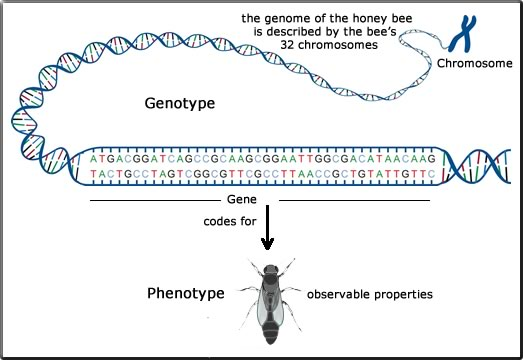
\includegraphics[width=0.5\linewidth]{figs/gene.jpg}\\
	\tiny \href{https://killowen.com/assets/phenotype.jpg}{(Source)}

	%\includegraphics[width=0.7\linewidth]{figs/exon.png}\\
	%\tiny \href{https://en.wikipedia.org/wiki/Exon}{(Source)}
	\end{center}
\end{frame}

\subsection{{Theory of Evolution from an algorithmic perspective}}
\begin{frame}{Biological background}{Theory of Evolution from an algorithmic perspective}
	Given a population ...
	\begin{enumerate}
	\item There are differences among individuals
	\item Fittest individuals are more likely to reproduce
	\item Good trails increase their presence in the population
	\item Go to 1
	\end{enumerate}
	We are interested in applying this to Engineering
\end{frame}

\begin{frame}[plain]{}
%	\note{Poner como ejemplo el perfil de un ala, geometria de una antena microscript, red neuronal e insercion orbital}
%	\vspace{2cm}
	\begin{center}
	How can we apply biological evolution to solve engineering problems?
	\end{center}
\end{frame}

\section{Evolutionary Algorithms}
\subsection{Evolution as optimization}
\begin{frame}{Evolutionary Algorithms}{Evolution as optimization}
    \begin{columns}
 	   \column{.50\textwidth}
	\begin{center}
	\includegraphics[width=\linewidth]{figs/fitness-landscape-0.png}\\
		\tiny \href{http://2.bp.blogspot.com/-32R9V6X6rXU/T-tr1lZIwCI/AAAAAAAAAFI/t05ioQ5GP80/s1600/Fitness-Landscape.gif}{(Source)}
	\end{center}
 	   \column{.50\textwidth}
	Biological evolution is, in essence, an optimization algorithm
	\begin{itemize}
	\item ... it optimizes the survival probability
	\item Optimizing is to \textit{search} the maximum
	\end{itemize}
	\end{columns}
\end{frame}

\subsection{AI, search and optimization}
%\begin{frame}{Introduction}{Motivation}
\begin{frame}{Evolutionary Algorithms}{AI, search and optimization (I)}
    \begin{columns}
 	   \column{.60\textwidth}

    %Early AI works were directed to
    %\begin{itemize}
    %    \item Proof of theorems, crosswords, games, ...
    %\end{itemize}

    All in AI is search ...
    \begin{itemize}
        \item ... not entirely true (obviously) but more than we may imagine
        \item Find a good/best solution (\alert{solution space}) to a problem among several potential solutions (\alert{search space})
    \end{itemize}

    Almost any AI problem can be expressed as a search problem

    %\textbf{Enhaustive search} (or brute-force search)
    %\begin{itemize}
    %    \item Iterate over all the potential solutions
    %    \item Unsuiteable for most real-world problems
    %\end{itemize}

 	\column{.40\textwidth}
    	 %rch
%%%%%%%%%%%%%%%%%%%%%%%%%%%%%%%%%%%%%%%%%%%%%%%%%%%%%%%%%%%%%%%%
% MUW Presentation
% LaTeX Template
% Version 1.0 (27/12/2016)
%
% License:
% CC BY-NC-SA 4.0 (http://creativecommons.org/licenses/by-nc-sa/3.0/)
%
% Created by:
% Nicolas Ballarini, CeMSIIS, Medical University of Vienna
% nicoballarini@gmail.com
% http://statistics.msi.meduniwien.ac.at/
%
% Customized for UAH by:
% David F. Barrero, Departamento de Automática, UAH
%%%%%%%%%%%%%%%%%%%%%%%%%%%%%%%%%%%%%%%%%%%%%%%%%%%%%%%%%%%%%%%%%

\documentclass[10pt,compress]{beamer} % Change 10pt to make fonts of a different size
\mode<presentation>

\usepackage[spanish]{babel}
\usepackage{fontspec}
\usepackage{tikz}
\usepackage{etoolbox}
\usepackage{xcolor}
\usepackage{xstring}
\usepackage{listings}

% Custom packages
\usepackage{tikz}
\usepackage{pgfplots}
\def\layersep{2.5cm}
\usetikzlibrary{matrix,chains,positioning,decorations.pathreplacing,arrows}

\definecolor{dkgreen}{rgb}{0,0.6,0}
\definecolor{gray}{rgb}{0.5,0.5,0.5}
\definecolor{mauve}{rgb}{0.58,0,0.82}
 

\usetheme{UAH}
\usecolortheme{UAH}
\setbeamertemplate{navigation symbols}{} 
\setbeamertemplate{caption}[numbered]

%%%%%%%%%%%%%%%%%%%%%%%%%%%%%%%%%%%%%%%%%%%%%%%%%%%%%%%%%%%%%%%%%
%% Presentation Info
\title[Search algorithm]{Solving Problems by Searching}
\author{\asignatura\\\carrera}
\institute{}
\date{Departamento de Automática}
%%%%%%%%%%%%%%%%%%%%%%%%%%%%%%%%%%%%%%%%%%%%%%%%%%%%%%%%%%%%%%%%%


%%%%%%%%%%%%%%%%%%%%%%%%%%%%%%%%%%%%%%%%%%%%%%%%%%%%%%%%%%%%%%%%%
%% Descomentar para habilitar barra de navegación superior
\setNavigation
%%%%%%%%%%%%%%%%%%%%%%%%%%%%%%%%%%%%%%%%%%%%%%%%%%%%%%%%%%%%%%%%%

%%%%%%%%%%%%%%%%%%%%%%%%%%%%%%%%%%%%%%%%%%%%%%%%%%%%%%%%%%%%%%%%%
%% Configuración de logotipos en portada
%% Opacidad de los logotipos
\newcommand{\opacidad}{1}
%% Descomentar para habilitar logotipo en pié de página de portada
\renewcommand{\logoUno}{Images/isg.png}
%% Descomentar para habilitar logotipo en pié de página de portada
%\renewcommand{\logoDos}{Images/CCLogo.png}
%% Descomentar para habilitar logotipo en pié de página de portada
%\renewcommand{\logoTres}{Images/ALogo.png}
%% Descomentar para habilitar logotipo en pié de página de portada
%\renewcommand{\logoCuatro}{Images/ELogo.png}
%%%%%%%%%%%%%%%%%%%%%%%%%%%%%%%%%%%%%%%%%%%%%%%%%%%%%%%%%%%%%%%%%

%%%%%%%%%%%%%%%%%%%%%%%%%%%%%%%%%%%%%%%%%%%%%%%%%%%%%%%%%%%%%%%%%
%% FOOTLINE
%% Comment/Uncomment the following blocks to modify the footline
%% content in the body slides. 


%% Option A: Title and institute
\footlineA
%% Option B: Author and institute
%\footlineB
%% Option C: Title, Author and institute
%\footlineC
%%%%%%%%%%%%%%%%%%%%%%%%%%%%%%%%%%%%%%%%%%%%%%%%%%%%%%%%%%%%%%%%%

\begin{document}

%%%%%%%%%%%%%%%%%%%%%%%%%%%%%%%%%%%%%%%%%%%%%%%%%%%%%%%%%%%%%%%%%
% Use this block for a blue title slide with modified footline
{\titlepageBlue
    \begin{frame}
        \titlepage
    \end{frame}
}

\institute{\asignatura}

\begin{frame}[plain]{}
   \begin{block}{Objectives}
      \begin{enumerate}
         \item Understand the role of search in AI
         \item Describe the importance of trees in search
         \item Express AI problems in terms of search
         \item Apply classical search algorithms
      \end{enumerate} 
   \end{block}

   \begin{block}{Bibliography}
	\begin{itemize}
        \item S. Russell and P. Norvig. Chapter 3, Solving Problems by Searching. \textit{Artificial Intelligence: A Modern Approach}. Pearson. 2017
	\end{itemize}
   \end{block}
\end{frame}

{
\disableNavigation{white}
\begin{frame}[shrink]{Table of Contents}
 \frametitle{Table of Contents}
 \tableofcontents
  % You might wish to add the option [pausesections]
\end{frame}
}

\section{Introduction}

\begin{frame}{Introduction}{Intelligent agent}
    \begin{columns}
 	   \column{.50\textwidth}
        \begin{block}{Agent}
        An agent is anything that can be viewed as perceiving its environment through sensors and acting through actuators
        \end{block}

 	   \column{.50\textwidth}
       \begin{center}
	        \includegraphics[width=0.9\linewidth]{figs/agent-environment.eps}\\
	        \tiny{\href{http://aima.cs.berkeley.edu/index.html}{(Source)}}
	    \end{center}

	\end{columns}

    \begin{itemize}
        \item Agents is a research field in AI by its own 
            \begin{itemize}
                \item ... with its own definition of agent (caution!)
            \end{itemize}
        \item We use this term to abstract the implementation
    \end{itemize}
\end{frame}

\begin{frame}{Introduction}{Motivation}

    \begin{columns}
 	   \column{.60\textwidth}

    Early AI works were directed to
    \begin{itemize}
        \item Proof of theorems, crosswords, games, ...
    \end{itemize}

    All in AI is search ...
    \begin{itemize}
        \item ... not entirely true (obviously) but more than we may imagine
        \item Find a good/best solution (\alert{solution space}) to a problem among several potential solutions (\alert{search space})
    \end{itemize}

    \textbf{Enhaustive search} (or brute-force search)
    \begin{itemize}
        \item Iterate over all the potential solutions
        \item Unsuiteable for most real-world problems
    \end{itemize}

 	\column{.40\textwidth}
     %rch
%%%%%%%%%%%%%%%%%%%%%%%%%%%%%%%%%%%%%%%%%%%%%%%%%%%%%%%%%%%%%%%%
% MUW Presentation
% LaTeX Template
% Version 1.0 (27/12/2016)
%
% License:
% CC BY-NC-SA 4.0 (http://creativecommons.org/licenses/by-nc-sa/3.0/)
%
% Created by:
% Nicolas Ballarini, CeMSIIS, Medical University of Vienna
% nicoballarini@gmail.com
% http://statistics.msi.meduniwien.ac.at/
%
% Customized for UAH by:
% David F. Barrero, Departamento de Automática, UAH
%%%%%%%%%%%%%%%%%%%%%%%%%%%%%%%%%%%%%%%%%%%%%%%%%%%%%%%%%%%%%%%%%

\documentclass[10pt,compress]{beamer} % Change 10pt to make fonts of a different size
\mode<presentation>

\usepackage[spanish]{babel}
\usepackage{fontspec}
\usepackage{tikz}
\usepackage{etoolbox}
\usepackage{xcolor}
\usepackage{xstring}
\usepackage{listings}

% Custom packages
\usepackage{tikz}
\usepackage{pgfplots}
\def\layersep{2.5cm}
\usetikzlibrary{matrix,chains,positioning,decorations.pathreplacing,arrows}

\definecolor{dkgreen}{rgb}{0,0.6,0}
\definecolor{gray}{rgb}{0.5,0.5,0.5}
\definecolor{mauve}{rgb}{0.58,0,0.82}
 

\usetheme{UAH}
\usecolortheme{UAH}
\setbeamertemplate{navigation symbols}{} 
\setbeamertemplate{caption}[numbered]

%%%%%%%%%%%%%%%%%%%%%%%%%%%%%%%%%%%%%%%%%%%%%%%%%%%%%%%%%%%%%%%%%
%% Presentation Info
\title[Search algorithm]{Solving Problems by Searching}
\author{\asignatura\\\carrera}
\institute{}
\date{Departamento de Automática}
%%%%%%%%%%%%%%%%%%%%%%%%%%%%%%%%%%%%%%%%%%%%%%%%%%%%%%%%%%%%%%%%%


%%%%%%%%%%%%%%%%%%%%%%%%%%%%%%%%%%%%%%%%%%%%%%%%%%%%%%%%%%%%%%%%%
%% Descomentar para habilitar barra de navegación superior
\setNavigation
%%%%%%%%%%%%%%%%%%%%%%%%%%%%%%%%%%%%%%%%%%%%%%%%%%%%%%%%%%%%%%%%%

%%%%%%%%%%%%%%%%%%%%%%%%%%%%%%%%%%%%%%%%%%%%%%%%%%%%%%%%%%%%%%%%%
%% Configuración de logotipos en portada
%% Opacidad de los logotipos
\newcommand{\opacidad}{1}
%% Descomentar para habilitar logotipo en pié de página de portada
\renewcommand{\logoUno}{Images/isg.png}
%% Descomentar para habilitar logotipo en pié de página de portada
%\renewcommand{\logoDos}{Images/CCLogo.png}
%% Descomentar para habilitar logotipo en pié de página de portada
%\renewcommand{\logoTres}{Images/ALogo.png}
%% Descomentar para habilitar logotipo en pié de página de portada
%\renewcommand{\logoCuatro}{Images/ELogo.png}
%%%%%%%%%%%%%%%%%%%%%%%%%%%%%%%%%%%%%%%%%%%%%%%%%%%%%%%%%%%%%%%%%

%%%%%%%%%%%%%%%%%%%%%%%%%%%%%%%%%%%%%%%%%%%%%%%%%%%%%%%%%%%%%%%%%
%% FOOTLINE
%% Comment/Uncomment the following blocks to modify the footline
%% content in the body slides. 


%% Option A: Title and institute
\footlineA
%% Option B: Author and institute
%\footlineB
%% Option C: Title, Author and institute
%\footlineC
%%%%%%%%%%%%%%%%%%%%%%%%%%%%%%%%%%%%%%%%%%%%%%%%%%%%%%%%%%%%%%%%%

\begin{document}

%%%%%%%%%%%%%%%%%%%%%%%%%%%%%%%%%%%%%%%%%%%%%%%%%%%%%%%%%%%%%%%%%
% Use this block for a blue title slide with modified footline
{\titlepageBlue
    \begin{frame}
        \titlepage
    \end{frame}
}

\institute{\asignatura}

\begin{frame}[plain]{}
   \begin{block}{Objectives}
      \begin{enumerate}
         \item Understand the role of search in AI
         \item Describe the importance of trees in search
         \item Express AI problems in terms of search
         \item Apply classical search algorithms
      \end{enumerate} 
   \end{block}

   \begin{block}{Bibliography}
	\begin{itemize}
        \item S. Russell and P. Norvig. Chapter 3, Solving Problems by Searching. \textit{Artificial Intelligence: A Modern Approach}. Pearson. 2017
	\end{itemize}
   \end{block}
\end{frame}

{
\disableNavigation{white}
\begin{frame}[shrink]{Table of Contents}
 \frametitle{Table of Contents}
 \tableofcontents
  % You might wish to add the option [pausesections]
\end{frame}
}

\section{Introduction}

\begin{frame}{Introduction}{Intelligent agent}
    \begin{columns}
 	   \column{.50\textwidth}
        \begin{block}{Agent}
        An agent is anything that can be viewed as perceiving its environment through sensors and acting through actuators
        \end{block}

 	   \column{.50\textwidth}
       \begin{center}
	        \includegraphics[width=0.9\linewidth]{figs/agent-environment.eps}\\
	        \tiny{\href{http://aima.cs.berkeley.edu/index.html}{(Source)}}
	    \end{center}

	\end{columns}

    \begin{itemize}
        \item Agents is a research field in AI by its own 
            \begin{itemize}
                \item ... with its own definition of agent (caution!)
            \end{itemize}
        \item We use this term to abstract the implementation
    \end{itemize}
\end{frame}

\begin{frame}{Introduction}{Motivation}

    \begin{columns}
 	   \column{.60\textwidth}

    Early AI works were directed to
    \begin{itemize}
        \item Proof of theorems, crosswords, games, ...
    \end{itemize}

    All in AI is search ...
    \begin{itemize}
        \item ... not entirely true (obviously) but more than we may imagine
        \item Find a good/best solution (\alert{solution space}) to a problem among several potential solutions (\alert{search space})
    \end{itemize}

    \textbf{Enhaustive search} (or brute-force search)
    \begin{itemize}
        \item Iterate over all the potential solutions
        \item Unsuiteable for most real-world problems
    \end{itemize}

 	\column{.40\textwidth}
     %rch
%%%%%%%%%%%%%%%%%%%%%%%%%%%%%%%%%%%%%%%%%%%%%%%%%%%%%%%%%%%%%%%%
% MUW Presentation
% LaTeX Template
% Version 1.0 (27/12/2016)
%
% License:
% CC BY-NC-SA 4.0 (http://creativecommons.org/licenses/by-nc-sa/3.0/)
%
% Created by:
% Nicolas Ballarini, CeMSIIS, Medical University of Vienna
% nicoballarini@gmail.com
% http://statistics.msi.meduniwien.ac.at/
%
% Customized for UAH by:
% David F. Barrero, Departamento de Automática, UAH
%%%%%%%%%%%%%%%%%%%%%%%%%%%%%%%%%%%%%%%%%%%%%%%%%%%%%%%%%%%%%%%%%

\documentclass[10pt,compress]{beamer} % Change 10pt to make fonts of a different size
\mode<presentation>

\usepackage[spanish]{babel}
\usepackage{fontspec}
\usepackage{tikz}
\usepackage{etoolbox}
\usepackage{xcolor}
\usepackage{xstring}
\usepackage{listings}

% Custom packages
\usepackage{tikz}
\usepackage{pgfplots}
\def\layersep{2.5cm}
\usetikzlibrary{matrix,chains,positioning,decorations.pathreplacing,arrows}

\definecolor{dkgreen}{rgb}{0,0.6,0}
\definecolor{gray}{rgb}{0.5,0.5,0.5}
\definecolor{mauve}{rgb}{0.58,0,0.82}
 

\usetheme{UAH}
\usecolortheme{UAH}
\setbeamertemplate{navigation symbols}{} 
\setbeamertemplate{caption}[numbered]

%%%%%%%%%%%%%%%%%%%%%%%%%%%%%%%%%%%%%%%%%%%%%%%%%%%%%%%%%%%%%%%%%
%% Presentation Info
\title[Search algorithm]{Solving Problems by Searching}
\author{\asignatura\\\carrera}
\institute{}
\date{Departamento de Automática}
%%%%%%%%%%%%%%%%%%%%%%%%%%%%%%%%%%%%%%%%%%%%%%%%%%%%%%%%%%%%%%%%%


%%%%%%%%%%%%%%%%%%%%%%%%%%%%%%%%%%%%%%%%%%%%%%%%%%%%%%%%%%%%%%%%%
%% Descomentar para habilitar barra de navegación superior
\setNavigation
%%%%%%%%%%%%%%%%%%%%%%%%%%%%%%%%%%%%%%%%%%%%%%%%%%%%%%%%%%%%%%%%%

%%%%%%%%%%%%%%%%%%%%%%%%%%%%%%%%%%%%%%%%%%%%%%%%%%%%%%%%%%%%%%%%%
%% Configuración de logotipos en portada
%% Opacidad de los logotipos
\newcommand{\opacidad}{1}
%% Descomentar para habilitar logotipo en pié de página de portada
\renewcommand{\logoUno}{Images/isg.png}
%% Descomentar para habilitar logotipo en pié de página de portada
%\renewcommand{\logoDos}{Images/CCLogo.png}
%% Descomentar para habilitar logotipo en pié de página de portada
%\renewcommand{\logoTres}{Images/ALogo.png}
%% Descomentar para habilitar logotipo en pié de página de portada
%\renewcommand{\logoCuatro}{Images/ELogo.png}
%%%%%%%%%%%%%%%%%%%%%%%%%%%%%%%%%%%%%%%%%%%%%%%%%%%%%%%%%%%%%%%%%

%%%%%%%%%%%%%%%%%%%%%%%%%%%%%%%%%%%%%%%%%%%%%%%%%%%%%%%%%%%%%%%%%
%% FOOTLINE
%% Comment/Uncomment the following blocks to modify the footline
%% content in the body slides. 


%% Option A: Title and institute
\footlineA
%% Option B: Author and institute
%\footlineB
%% Option C: Title, Author and institute
%\footlineC
%%%%%%%%%%%%%%%%%%%%%%%%%%%%%%%%%%%%%%%%%%%%%%%%%%%%%%%%%%%%%%%%%

\begin{document}

%%%%%%%%%%%%%%%%%%%%%%%%%%%%%%%%%%%%%%%%%%%%%%%%%%%%%%%%%%%%%%%%%
% Use this block for a blue title slide with modified footline
{\titlepageBlue
    \begin{frame}
        \titlepage
    \end{frame}
}

\institute{\asignatura}

\begin{frame}[plain]{}
   \begin{block}{Objectives}
      \begin{enumerate}
         \item Understand the role of search in AI
         \item Describe the importance of trees in search
         \item Express AI problems in terms of search
         \item Apply classical search algorithms
      \end{enumerate} 
   \end{block}

   \begin{block}{Bibliography}
	\begin{itemize}
        \item S. Russell and P. Norvig. Chapter 3, Solving Problems by Searching. \textit{Artificial Intelligence: A Modern Approach}. Pearson. 2017
	\end{itemize}
   \end{block}
\end{frame}

{
\disableNavigation{white}
\begin{frame}[shrink]{Table of Contents}
 \frametitle{Table of Contents}
 \tableofcontents
  % You might wish to add the option [pausesections]
\end{frame}
}

\section{Introduction}

\begin{frame}{Introduction}{Intelligent agent}
    \begin{columns}
 	   \column{.50\textwidth}
        \begin{block}{Agent}
        An agent is anything that can be viewed as perceiving its environment through sensors and acting through actuators
        \end{block}

 	   \column{.50\textwidth}
       \begin{center}
	        \includegraphics[width=0.9\linewidth]{figs/agent-environment.eps}\\
	        \tiny{\href{http://aima.cs.berkeley.edu/index.html}{(Source)}}
	    \end{center}

	\end{columns}

    \begin{itemize}
        \item Agents is a research field in AI by its own 
            \begin{itemize}
                \item ... with its own definition of agent (caution!)
            \end{itemize}
        \item We use this term to abstract the implementation
    \end{itemize}
\end{frame}

\begin{frame}{Introduction}{Motivation}

    \begin{columns}
 	   \column{.60\textwidth}

    Early AI works were directed to
    \begin{itemize}
        \item Proof of theorems, crosswords, games, ...
    \end{itemize}

    All in AI is search ...
    \begin{itemize}
        \item ... not entirely true (obviously) but more than we may imagine
        \item Find a good/best solution (\alert{solution space}) to a problem among several potential solutions (\alert{search space})
    \end{itemize}

    \textbf{Enhaustive search} (or brute-force search)
    \begin{itemize}
        \item Iterate over all the potential solutions
        \item Unsuiteable for most real-world problems
    \end{itemize}

 	\column{.40\textwidth}
     \input{figs/search.tex}
    \end{columns}
\end{frame}

\section{Problem formulation}
\subsection{Types of problems}
\begin{frame}{Problem formulation}{Types of problems}
    %Search is a cornerstone in AI
    %\begin{itemize}
    %    \item Almost any problem in AI is formulated as a search problem
    %\end{itemize}

    Types of problems depending on ...
	\begin{itemize}
        \item Knowledge
            \begin{itemize}
                \item[-] Observable or Non-observable or Partially observable
            \end{itemize}
        \item Outcome
            \begin{itemize}
                \item[-] Deterministic or Stochastic
            \end{itemize}
        \item Actions
            \begin{itemize}
                \item[-] Discrete or Continous
            \end{itemize}
        \item Time-variance
            \begin{itemize}
                \item[-] Static or Dynamic
            \end{itemize}
	\end{itemize}
    We assume static, observable, discrete and deterministic problems
\end{frame}

\begin{frame}[fragile]{Problem formulation}{Types of problems (II)}
    \begin{exampleblock}{Determine problem type}
       \begin{columns}
 	       \column{.50\textwidth}
           \centering Chess\\
           \medskip
	        \includegraphics[width=0.75\linewidth]{figs/chess.png}\\

 	       \column{.50\textwidth}
           \centering League of Legends\\
           \medskip
	        \includegraphics[width=0.75\linewidth]{figs/lol.jpg}\\
        \end{columns}
        \medskip
        Observable or non-observable, deterministic or stochastic, discrete or continous, static or dynamic?
    \end{exampleblock}
\end{frame}

\subsection{Problem components}
\begin{frame}{Problem formulation}{Problem components (I)}
    We represent the environment as \alert{states}
        \begin{itemize}
            \item Contain the information about the world
        \end{itemize}
    Any problem formulation requires the following components
	\begin{itemize}
        \item \textbf{Initial state}: State where the search begins
        \item \textbf{Actions}: Behaviour that the agent may exhibit
        \item \textbf{Transition model}: Which states follow an action in a state (\alert{graph})
        \item \textbf{Goal test} (\textit{metas}): How to determine if a state is a goal
        \item \textbf{Path cost}: Cost of a path to a state
	\end{itemize}
\end{frame}

\begin{frame}{Problem formulation}{Problem components: Example (I)}
    \begin{center}
	    \includegraphics[width=0.7\linewidth]{figs/romania-distances.eps}\\
	    \tiny{\href{http://aima.cs.berkeley.edu/index.html}{(Source)}}
	\end{center}

    \begin{exampleblock}{Problem: Move from Arad to Bucharest}
        On holiday in Romania; currently in Arad, flight leaves tomorrow from Bucharest\\
        Determine: Initial state, goal, states, actions, transition model, goal test and path cost
    \end{exampleblock}
\end{frame}

\begin{frame}{Problem formulation}{Problem components: Example (II)}

       \begin{columns}
 	       \column{.60\textwidth}
    \begin{center}
	    \includegraphics[width=\linewidth]{figs/romania-distances.eps}\\
	    \tiny{\href{http://aima.cs.berkeley.edu/index.html}{(Source)}}
	\end{center}

 	       \column{.50\textwidth}
    \begin{exampleblock}{Solution}
        \begin{itemize}
            \item Initial state: Arad
            \item Goal: Bucharest
            \item States: Multiple cities
            \item Actions: Drive between cities
            \item Goal test: In Bucharest?
            \item Path cost: Distance
        \end{itemize}
    \end{exampleblock}

       \end{columns}
\end{frame}

\begin{frame}{Problem formulation}{Problem components: Search}
    \alert{Search} is the process of finding a solution
        \begin{itemize}
            \item A \alert{solution} is a sequence of actions leading from the initial state to a goal state
            \item \alert{Optimal solution} is a solution with the lowest cost
            \item Example of solution: Arad $\rightarrow$ Sibiu $\rightarrow$ Fagaras $\rightarrow$ Bucharest
                \begin{itemize}
                \item That solution is optimal?
                \end{itemize}
        \end{itemize}
\end{frame}


\subsection{Toy problems}
\begin{frame}[fragile]{Search problems}{Toy problems (I): Vacuum world}
       \begin{columns}
 	       \column{.40\textwidth}
	            \centering 
                \onslide<1> \includegraphics[width=\linewidth]{figs/vacuum2-environment.eps}\\
	            \tiny{\href{http://aima.cs.berkeley.edu/index.html}{(Source)}}

 	       \column{.60\textwidth}
                \begin{exampleblock}{Problem: Clean rooms}
                    \begin{itemize}
                    \item[-] State? $\rightarrow$ 
                    \item[-] Initial state? $\rightarrow$ 
                    \item[-] Goal? $\rightarrow$ 
                    \item[-] Actions? $\rightarrow$ 
                    \item[-] Transition model? $\rightarrow$ 
                    \item[-] Goal test? $\rightarrow$ 
                    \item[-] Path cost? $\rightarrow$
                    \end{itemize}
                \end{exampleblock}
      \end{columns}
\end{frame}

\begin{frame}[fragile]{Search problems}{Toy problems (I): Vacuum world}
       \begin{columns}
 	       \column{.40\textwidth}
	           \centering 
               \includegraphics[width=\linewidth]{figs/vacuum2-state-space.eps}\\
	           \tiny{\href{http://aima.cs.berkeley.edu/index.html}{(Source)}}

 	       \column{.60\textwidth}
                \begin{exampleblock}{Problem: Clean rooms}
                    \begin{itemize}
                    \item[-] State? $\rightarrow$ \textit{Dirt and location}
                    \item[-] Initial state? $\rightarrow$ \textit{All dirt, Left}
                    \item[-] Goal? $\rightarrow$ \textit{No dirt, any location}
                    \item[-] Actions? $\rightarrow$ \textit{Left, Right, Suck}
                    \item[-] Transition model? $\rightarrow$ \textit{See figure}
                    \item[-] Goal test? $\rightarrow$ \textit{No dirt, any location}
                    \item[-] Path cost? $\rightarrow$ \textit{1 per action}
                    \end{itemize}
                \end{exampleblock}
      \end{columns}
\end{frame}

\begin{frame}{Search problems}{Toy problems (II): 8-puzzle}
       \begin{columns}
 	       \column{.40\textwidth}
	            \centering \includegraphics[width=\linewidth]{figs/8puzzle.eps}\\
	            \tiny{\href{http://aima.cs.berkeley.edu/index.html}{(Source)}}
 	       \column{.60\textwidth}
                \begin{exampleblock}{Problem: Solve 8-puzzle}
                    \begin{itemize}
                    \item[-] State? $\rightarrow$ 
                    \item[-] Initial state? $\rightarrow$ 
                    \item[-] Goal? $\rightarrow$ 
                    \item[-] Actions? $\rightarrow$ 
                    \item[-] Transition model? $\rightarrow$ 
                    \item[-] Goal test? $\rightarrow$ 
                    \item[-] Path cost? $\rightarrow$
                    \end{itemize}
                \end{exampleblock}
      \end{columns}
\end{frame}

\begin{frame}{Search problems}{Toy problems (II): 8-puzzle}
       \begin{columns}
 	       \column{.40\textwidth}
	            \centering \includegraphics[width=\linewidth]{figs/8puzzle.eps}\\
	            \tiny{\href{http://aima.cs.berkeley.edu/index.html}{(Source)}}
 	       \column{.60\textwidth}
                \begin{exampleblock}{Problem: Solve 8-puzzle}
                    \begin{itemize}
                    \item[-] State? $\rightarrow$ \textit{Location of tiles}
                        \begin{itemize}
                            \item[] $9!/2 = 181,440$ states
                        \end{itemize}
                    \item[-] Initial state? $\rightarrow$ \textit{Any}
                    \item[-] Goal? $\rightarrow$ \textit{See figure}
                    \item[-] Actions? $\rightarrow$ \textit{Left, Right, Up, Down}
                    \item[-] Transition model? $\rightarrow$ Complex graph
                    \item[-] Goal test? $\rightarrow$ \textit{Goal state}
                    \item[-] Path cost? $\rightarrow$ \textit{1 per move}
                    \end{itemize}
                \end{exampleblock}

      \end{columns}
\end{frame}

\begin{frame}{Search problems}{Toy problems (III): 8-queens}
       \begin{columns}
 	       \column{.40\textwidth}
	            \centering \includegraphics[width=\linewidth]{figs/8queens.eps}\\
	            \tiny{\href{http://aima.cs.berkeley.edu/index.html}{(Source)}}
 	       \column{.60\textwidth}
                \begin{exampleblock}{Problem: Place 8 queens no queen attacks any other}
                State?\\
                Initial state? \\
                Goal? \\
                Actions? \\ 
                Transition model? \\
                Goal test? \\
                Path cost?\\
                \end{exampleblock}
      \end{columns}
\end{frame}

\begin{frame}{Search problems}{Toy problems (III): 8-queens}
       \begin{columns}
 	       \column{.40\textwidth}
	            \centering \includegraphics[width=\linewidth]{figs/8queens.eps}\\
	            \tiny{\href{http://aima.cs.berkeley.edu/index.html}{(Source)}}
 	       \column{.60\textwidth}
                \begin{exampleblock}{Problem: Place 8 queens no queen attacks any other}
                    \begin{itemize}
                    \item[-] State? $\rightarrow$ \textit{Any arrangement of 0 to 8 queens}
                    \item[-] Initial state? $\rightarrow$ \textit{Empty board}
                    \item[-] Goal? $\rightarrow$ \textit{See figure}
                    \item[-] Actions? $\rightarrow$ \textit{Add queen to empty square}
                    \item[-] Transition model? $\rightarrow$ Complex graph
                    \item[-] Goal test? $\rightarrow$ \textit{8 queens on board, none attacked}
                    \item[-] Path cost? $\rightarrow$ \textit{1 per move}
                    \end{itemize}
                \end{exampleblock}
      \end{columns}
\end{frame}

\subsection{Travel Salesman Problem}
\begin{frame}{Search problems}{Travelling Salesman Problem (TSP)}
       \begin{columns}
 	       \column{.50\textwidth}
                \begin{block}{TSP formulation}
                    A travelling salesman must visit a set of cities only one time each. Find the shortest route.
                \end{block}

                TSP is a very big problem in AI!
                \begin{itemize}
                    \item First formulated in 1930 and still a hot research topic!
                    \item NP-hard problem
                    \item Many real world applications
                \end{itemize}

 	       \column{.50\textwidth}
                \centering 
                \begin{tikzpicture}[scale=0.6]
                    \node[shape=circle, draw] (A) at (0,0) {A};
                    \node[shape=circle, draw] (B) at (0,3) {B};
                    \node[shape=circle, draw] (C) at (2.5,4) {C};
                    \node[shape=circle, draw] (D) at (2.5,1) {D};
                    \node[shape=circle, draw] (E) at (2.5,-2) {E};
                    \node[shape=circle, draw] (F) at (5,3) {F} ;

                    \path [-] (A) edge node[left] {$5$} (B);
                    \path [-](B) edge node[left] {$3$} (C);
                    \path [-](A) edge node[left] {$4$} (D);
                    \path [-](D) edge node[left] {$3$} (C);
                    \path [-](A) edge node[right] {$3$} (E);
                    \path [-](D) edge node[left] {$3$} (E);
                    \path [-](D) edge node {$3$} (F);
                    \path [-](C) edge node {$5$} (F);
                    \path [-](E) edge node[right] {$8$} (F); 
                \end{tikzpicture}

                \tiny{\href{https://tex.stackexchange.com/questions/270543/draw-a-graph-in-latex-with-tikz}{(Source)}}
      \end{columns}
\end{frame}

\section{Search strategy}

\begin{frame}{Search strategy (I)}
    In general ...
	    \begin{itemize}
    	    \item Each problem has a search graph, or \textbf{state space}
        	\item Searching means finding a path from the initial state to a goal state
    	\end{itemize}

    Basic idea
        \begin{itemize}
            \item Explore search space
            \item Generate a \textbf{search tree} (i.e., \textbf{expanding nodes})
        \end{itemize}

    A search strategy is defined by picking the order of node exansion
        \begin{itemize}
            \item Uninformed search: Only uses the problem definition
            \item Informed search: Uses problem-specific knowledge
        \end{itemize}
\end{frame}

\begin{frame}{Search strategy (II)}
    Search strategies are evaluated along the following dimensions
	    \begin{itemize}
    	    \item Completeness
        	\item Time complexity
            \item Space complexity
            \item Optimality
    	\end{itemize}

    Time and space are measured in terms of 
        \begin{itemize}
            \item b: Maximum branching factor
            \item d: Depth of the least-cost solution
            \item m: Maximum depth of the state space
        \end{itemize}
\end{frame}

\section{Uninformed search}
%\subsection{Introduction}

\begin{frame}{Uninformed search}
    Uninformed search algorithms
    \begin{itemize}
        \item Breadth-first search (\textit{búsqueda en anchura})
        \item Uniform-cost search (\textit{búsqueda de coste uniforme})
        \item Depth-first search (\textit{búsqueda en profundidad})
        \item Depth-limited search (\textit{búsqueda en profundidad limitada})
        \item Iterative deepening search (\textit{búsqueda de profundización iterativa})
    \end{itemize}
\end{frame}

\subsection{Breadth-first search}

\begin{frame}{Uninformed search}{Breadth-first search (I)}
      Expand shallowest unexpanded node
      \begin{itemize}
        \item Implemented with a FIFO queue (First-In First-Out)
      \end{itemize}

      \bigskip 

      \begin{center}
          \includegraphics[width=\linewidth]{figs/bfs-progress.eps}\\
          \tiny{\href{http://aima.cs.berkeley.edu/index.html}{(Source)}}
      \end{center}
\end{frame}

\begin{frame}{Uninformed search}{Breadth-first search (II)}
      \begin{center}
          \setlength{\fboxrule}{0pt}
          \fbox{\includegraphics[natwidth=1124bp,natheight=462bp, width=0.7\linewidth]{figs/20-Figure3.13-1.png}} \\
          %\includegraphics[natwidth=1124, natwidth=462]{figs/20-Figure3.13-1.png}\\
          \tiny{\href{http://aima.cs.berkeley.edu/index.html}{(Source)}}
      \end{center}

      \bigskip

      Properties of breadth-first search
      \begin{itemize}
        \item Completeness: Yes
        \item Time complexity: $O(b^{d+1})$
        \item Space complexity: $O(b^{d+1})$
        \item Optimality: Yes (if cost = 1 per step)
      \end{itemize}
      Space is the biggest problem (more than time)
\end{frame}

\subsection{Uniform-cost search}

\begin{frame}{Uninformed search}{Uniform-cost search (I)}
    Special case of breadth-first search
    \begin{itemize}
        \item Expand least-cost unexpanded node
        \item The queue is sorted by cost
    \end{itemize}

    \begin{columns}
 	       \column{.50\textwidth}
                \setlength{\fboxrule}{0pt}
                \fbox{\includegraphics[width=\linewidth]{figs/Grafo1.png}} 
 	       \column{.50\textwidth}
                \setlength{\fboxrule}{0pt}
                \fbox{\includegraphics[width=0.7\linewidth]{figs/Grafo2.png}} 
    \end{columns}
\end{frame}

\begin{frame}[fragile]{Uninformed search}{Uniform-cost search (II)}
    \begin{exampleblock}{Uniform-cost example}
    \small{
    Initialization: $\{[S, 0]\}$\\
    Iter. 1: $\{[S \rightarrow A, 1], [S \rightarrow G, 12]\}$\\
    Iter. 2: $\{[S \rightarrow A \rightarrow C, 2], [S \rightarrow A \rightarrow B, 4], [S \rightarrow G, 12]\}$\\
    Iter. 3: $\{[S \rightarrow A \rightarrow C \rightarrow D, 3], [S \rightarrow A \rightarrow C \rightarrow G, 4], [S \rightarrow A \rightarrow B \rightarrow D, 7], [S \rightarrow G, 12]\}$\\
    Iter. 4: $\{[S \rightarrow A \rightarrow C \rightarrow D \rightarrow G, 6], [S \rightarrow A \rightarrow C \rightarrow G, 4], [S \rightarrow A \rightarrow B \rightarrow D, 7], [S \rightarrow G, 12]\}$\\
    Iter. 5: $\{[S \rightarrow A \rightarrow C \rightarrow G, 4], [S \rightarrow A \rightarrow C \rightarrow D \rightarrow G, 10], [S \rightarrow G, 12]\}$\\
    Solution: $S \rightarrow A \rightarrow C \rightarrow G$\\
    }
    \end{exampleblock}
\end{frame}

\begin{frame}[fragile]{Uninformed search}{Uniform-cost search (III)}
      Properties
      \begin{itemize}
        \item Completeness: Yes, if step cost $\ge\epsilon$
        \item Time complexity: $O(b^{\lceil C^{*}/\epsilon \rceil})$, where $C^{*}$ is the cost of the optimal solution
        \item Space complexity: $O(b^{\lceil C^{*}/\epsilon \rceil})$
        \item Optimality: Yes
      \end{itemize}
      Space is the biggest problem (more than time)
\end{frame}

\subsection{Depth-first search}

\begin{frame}{Uninformed search}{Depth-first search (I)}
    Expand deepest unexpanded node
    \begin{itemize}
        \item Implemented with a LIFO stack
    \end{itemize}
\end{frame}

\begin{frame}[plain]
      \begin{center}
          \includegraphics[width=\linewidth]{figs/dfs-progress-noblack.eps}\\
          \tiny{\href{http://aima.cs.berkeley.edu/index.html}{(Source)}}
      \end{center}
\end{frame}

\begin{frame}{Uninformed search}{Depth-first search (III)}
      Properties of depth-first search
      \begin{itemize}
        \item Completeness: No, fail in infinite-depth spaces or spaces with loops
        \item Time complexity: $O(b^{m})$, (terrible if $m>>d$)
        \item Space complexity: $O(bm)$
        \item Optimality: No
      \end{itemize}
\end{frame}

\subsection{Depth-limited search}

\begin{frame}{Uninformed search}{Depth-limited search}
      Depth-first search with depth limit L
      \begin{itemize}
        \item Nodes at depth L are not expanded
      \end{itemize}
\end{frame}

\subsection{Iterative deepening depth-first search}

\begin{frame}{Uninformed search}{Iterative deepening depth-first search (I)}
    Depth-limited search where gradually increases L
\end{frame}

\begin{frame}[plain,shrink]
      \begin{center}
          \includegraphics[width=\linewidth]{figs/ids-progress.eps}\\
          \tiny{\href{http://aima.cs.berkeley.edu/index.html}{(Source)}}
      \end{center}
\end{frame}

\begin{frame}{Uninformed search}{Iterative deepening depth-first search (III)}
      Properties
      \begin{itemize}
        \item Completeness: Yes
        \item Time complexity: $O(b^{d})$
        \item Space complexity: $O(bd)$
        \item Optimality: Yes if step cost = 1
      \end{itemize}
\end{frame}


\subsection{Comparison of uninformed search algorithms}

\begin{frame}{Uninformed search}{Comparison of uninformed search algorithms}

\begin{tabular}{cccccc}
\hline
Criterion & Breadth- & Uniform- & Depth- & Depth- & Iterative \\
          & First &  Cost & First & Limited & Deepening \\
\hline
Complete  & Yes$^*$ & Yes$^*$ & No & Yes, if $l \ge d$ & Yes \\
Time      & $b^{d+1}$ & $b^{\lceil C^*/\epsilon \rceil}$ & $b^m$ & $b^l$ & $b^d$ \\
Space     & $b^{d+1}$ & $b^{\lceil C^*/\epsilon \rceil}$ & $bm$ & $bl$ & $bd$ \\
Optimal   & Yes$^*$ & Yes & No & No & Yes$^*$ \\
\hline
\end{tabular}

\end{frame}


\section{Informed search}
\subsection{Introduction}

\begin{frame}{Informed search}{Introduction (I)}
    Use problem-specific knowledge beyond problem definition
      \begin{itemize}
        \item Best-first search (\textit{búsqueda primero el mejor})
            \begin{itemize}
                \item Greedy best-first search (\textit{Búsqueda voraz})
                \item A* search
            \end{itemize}
        \item Local search algorithms
            \begin{itemize}
            \item Hill-climbing search (\textit{búsqueda en escalada})
            \item Simulated annealing search (\textit{búsqueda de temple simulado})
            \item Local beam search (\textit{búsqueda de haz local})
            \item Genetic Algorithms 
        \end{itemize}
      \end{itemize}
\end{frame}

\begin{frame}{Informed search}{Introduction (II)}
    Best-first search
      \begin{itemize}
        \item Use an evaluation function $f(n)$ for each node
        \item Estimate of ``desirability''
        \item Expand most desirable unexpanded nodes
      \end{itemize}

    Most algorithms use a \alert{heuristic function} or just \alert{heuristic} ($h(n)$)
      \begin{itemize}
        \item Estimated cost from a state to the goal
      \end{itemize}

    Best-first algorithms
      \begin{itemize}
        \item Greedy best-first search
        \item A*
      \end{itemize}
\end{frame}

\subsection{Greedy best-first search}

\begin{frame}{Informed search}{Greedy best-first search (I)}
    \begin{columns}
 	    \column{.50\textwidth}
            It only considers the heuristic
            \begin{itemize}
                \item Greedy search expands the node that \textit{appears} to be closest to the goal
            \end{itemize}

 	    \column{.50\textwidth}
            \begin{block}{Greedy search}
                $f(n) = h (n)$
            \end{block}
    \end{columns}
    
    \bigskip

    Example: Find a path between Arad and Bucharest
    \begin{itemize}
        \item Heuristic: Straight-line distance
    \end{itemize}

    \centering \includegraphics[width=0.6\linewidth]{figs/romania-distances.eps}\\
    \tiny{\href{http://aima.cs.berkeley.edu/index.html}{(Source)}}
\end{frame}

\begin{frame}[plain,shrink]
      \begin{center}
          \includegraphics[width=\linewidth]{figs/greedy-progress.eps}\\
          \tiny{\href{http://aima.cs.berkeley.edu/index.html}{(Source)}}
      \end{center}
\end{frame}

\subsection{A*}

\begin{frame}{Informed search}{A* (I)}
    \begin{columns}
 	    \column{.50\textwidth}
            It considers the heuristic and the cost
            \begin{itemize}
                \item $h(n)$: Estimated cost to goal from node n
                \item $g(n)$: Cost to node n
            \end{itemize}

 	    \column{.50\textwidth}
            \begin{block}{A*}
                $f(n) = g(n) + h (n)$
            \end{block}
    \end{columns}

    \bigskip

    Theorem: A* is optimal if $h(n)$ is \alert{admisible}
        \begin{itemize}
        \item A* is admisible if it never overestimates the cost
        \item Example: Straight-line distance never overestimates road distance
        \end{itemize}
    \bigskip
\end{frame}

\begin{frame}[plain,shrink]
      \begin{center}
          \quad \includegraphics[width=\linewidth]{figs/astar-progress.eps}\\
          \tiny{\href{http://aima.cs.berkeley.edu/index.html}{(Source)}}
      \end{center}
\end{frame}

\begin{frame}{Informed search}{A* (III)}
      Properties
      \begin{itemize}
        \item Completeness: Yes
        \item Time complexity: Exponential
        \item Space complexity: Keeps all nodes in memory
        \item Optimality: Yes
      \end{itemize}
\end{frame}

\section{Case studies}
%\subsection{Case study I: Robotic assembly}

%\begin{frame}{Case studies}{Case study I: Robotic assembly}
%       \begin{columns}
%	       \column{.60\textwidth}
%            \centering \includegraphics[width=\linewidth]{figs/stanford-arm.eps}\\
%            \tiny{\href{http://aima.cs.berkeley.edu/index.html}{(Source)}}
%	       \column{.40\textwidth}
%               \begin{exampleblock}{Problem: Robotic assembly}
%                   \begin{itemize}
%                   \item[-] State? $\rightarrow$ \textit{Real-valued coordinates of robot joint angles}
%                   \item[-] Actions? $\rightarrow$ \textit{Continuous motions of joints}
%                   \item[-] Goal test? $\rightarrow$ \textit{Complete assembly}
%                   \item[-] Path cost? $\rightarrow$ \textit{Time to complete}
%                   \end{itemize}
%               \end{exampleblock}

%     \end{columns}
%end{frame}

\subsection{Case study I: Robot arm with two DOF}
\begin{frame}{Case studies}{Case study I: Robot arm with two DOF (I)}
       \begin{columns}
 	       \column{.50\textwidth}
	            \centering \includegraphics[width=\linewidth]{figs/armPlain.eps}\\
	            \tiny{\href{http://aima.cs.berkeley.edu/index.html}{(Source)}}
 	       \column{.50\textwidth}
                \begin{exampleblock}{Problem: Move arm}
                    \begin{itemize}
                    \item[-] State? $\rightarrow$ 
                    \item[-] Actions? $\rightarrow$ 
                    \item[-] Goal test? $\rightarrow$ 
                    \item[-] Path cost? $\rightarrow$
                    \end{itemize}
                \end{exampleblock}
      \end{columns}
\end{frame}

\begin{frame}{Case studies}{Case study I: Robot arm with two DOF (I)}
       \begin{columns}
 	       \column{.50\textwidth}
	            \centering \includegraphics[width=\linewidth]{figs/armPlain.eps}\\
	            \tiny{\href{http://aima.cs.berkeley.edu/index.html}{(Source)}}
 	       \column{.50\textwidth}
                \begin{exampleblock}{Problem: Move arm}
                    \begin{itemize}
                    \item[-] State? $\rightarrow$ \textit{Real-valued coordinates of robot joint angles}
                    \item[-] Actions? $\rightarrow$ \textit{Continuous motions of joints}
                    \item[-] Goal test? $\rightarrow$ \textit{Complete assembly}
                    \item[-] Path cost? $\rightarrow$ \textit{Time to complete}
                    \end{itemize}
                \end{exampleblock}
      \end{columns}
\end{frame}



\begin{frame}{Case studies}{Case study I: Robot arm with two DOF (II)}
       \begin{columns}
 	       \column{.50\textwidth}
            \centering \includegraphics[width=\linewidth]{figs/armPlain.eps}\\
	       \column{.50\textwidth}
            \centering \includegraphics[width=\linewidth]{figs/armPlainConfSpace.eps}\\
     \end{columns}
  \centering \tiny{\href{http://aima.cs.berkeley.edu/index.html}{(Source)}}
\end{frame}

\begin{frame}{Case studies}{Case study I: Robot arm with two DOF (III)}
       \begin{columns}
 	       \column{.50\textwidth}
	            \centering \includegraphics[width=\linewidth]{figs/armExampleWorkSpace.eps}\\
 	       \column{.50\textwidth}
	            \centering \includegraphics[width=\linewidth]{figs/armExampleConfSpace.eps}\\
      \end{columns}
	  \centering \tiny{\href{http://aima.cs.berkeley.edu/index.html}{(Source)}}
\end{frame}

\begin{frame}{Case studies}{Case study I: Robot arm with two DOF (IV)}
       \begin{columns}
 	       \column{.50\textwidth}
	            \centering \includegraphics[width=\linewidth]{figs/armDPwithoutPotentialWorkspaceCoarse.eps}\\
 	       \column{.50\textwidth}
	            \centering \includegraphics[width=\linewidth]{figs/armDPwithoutPotentialCoarse.eps}\\
      \end{columns}
	  \centering \tiny{\href{http://aima.cs.berkeley.edu/index.html}{(Source)}}
\end{frame}

\subsection{Case study II: 9\textsuperscript{th} GTOC}
\begin{frame}{Study case}{Case study II: 9\textsuperscript{th} Global Trajectory Optimization Competition (I)}
    GTOC: Global Trajectory Optimization Competition
    \begin{itemize}
        \item Proposed by ESA Advanced Concepts Team
        \item Difficult trajectory optimization problems
    \end{itemize}

    GTOC 9: The Kesser Run
    \begin{itemize}
        \item 123 orbiting debris
        \item Remove debris
        \item Design multiple missions
    \end{itemize}
    \href{https://www.youtube.com/watch?v=zvxZx-QnqQ0}{(Video)}
    \href{https://www.youtube.com/watch?v=5CQNG6OIbZM}{(Solution)}
\end{frame}

\subsection{Case study III: Mars orbital insertion}
\begin{frame}{Study case}{Case study III: Mars orbital insertion}
    \setlength{\fboxrule}{0pt}
    \fbox{\includegraphics[width=0.7\linewidth]{figs/orbits.jpg}} 
\end{frame}

\subsection{Case study IV: Transonic wing shape optimization}
\begin{frame}{Study case}{Case study IV: Transonic wing shape optimization}
    Problem: Design a wing shape for transonic flight
        \begin{itemize}
        \item Maximize lift
        \end{itemize}

    \setlength{\fboxrule}{0pt}
    \centering \fbox{\includegraphics[width=0.5\linewidth]{figs/wing-ga.png}} 
    
    \small
    \begin{flushleft}
    \href{https://link.springer.com/chapter/10.1007/978-94-010-0017-8\_38\#citeas}{Holst T.L., Pulliam T.H. (2003) \textit{Transonic Wing Shape Optimization Using a Genetic Algorithm}. In: IUTAM Symposium Transsonicum IV. Fluid Mechanics and its Applications, vol 73. Springer.}
    \end{flushleft}
\end{frame}

\end{document}

    \end{columns}
\end{frame}

\section{Problem formulation}
\subsection{Types of problems}
\begin{frame}{Problem formulation}{Types of problems}
    %Search is a cornerstone in AI
    %\begin{itemize}
    %    \item Almost any problem in AI is formulated as a search problem
    %\end{itemize}

    Types of problems depending on ...
	\begin{itemize}
        \item Knowledge
            \begin{itemize}
                \item[-] Observable or Non-observable or Partially observable
            \end{itemize}
        \item Outcome
            \begin{itemize}
                \item[-] Deterministic or Stochastic
            \end{itemize}
        \item Actions
            \begin{itemize}
                \item[-] Discrete or Continous
            \end{itemize}
        \item Time-variance
            \begin{itemize}
                \item[-] Static or Dynamic
            \end{itemize}
	\end{itemize}
    We assume static, observable, discrete and deterministic problems
\end{frame}

\begin{frame}[fragile]{Problem formulation}{Types of problems (II)}
    \begin{exampleblock}{Determine problem type}
       \begin{columns}
 	       \column{.50\textwidth}
           \centering Chess\\
           \medskip
	        \includegraphics[width=0.75\linewidth]{figs/chess.png}\\

 	       \column{.50\textwidth}
           \centering League of Legends\\
           \medskip
	        \includegraphics[width=0.75\linewidth]{figs/lol.jpg}\\
        \end{columns}
        \medskip
        Observable or non-observable, deterministic or stochastic, discrete or continous, static or dynamic?
    \end{exampleblock}
\end{frame}

\subsection{Problem components}
\begin{frame}{Problem formulation}{Problem components (I)}
    We represent the environment as \alert{states}
        \begin{itemize}
            \item Contain the information about the world
        \end{itemize}
    Any problem formulation requires the following components
	\begin{itemize}
        \item \textbf{Initial state}: State where the search begins
        \item \textbf{Actions}: Behaviour that the agent may exhibit
        \item \textbf{Transition model}: Which states follow an action in a state (\alert{graph})
        \item \textbf{Goal test} (\textit{metas}): How to determine if a state is a goal
        \item \textbf{Path cost}: Cost of a path to a state
	\end{itemize}
\end{frame}

\begin{frame}{Problem formulation}{Problem components: Example (I)}
    \begin{center}
	    \includegraphics[width=0.7\linewidth]{figs/romania-distances.eps}\\
	    \tiny{\href{http://aima.cs.berkeley.edu/index.html}{(Source)}}
	\end{center}

    \begin{exampleblock}{Problem: Move from Arad to Bucharest}
        On holiday in Romania; currently in Arad, flight leaves tomorrow from Bucharest\\
        Determine: Initial state, goal, states, actions, transition model, goal test and path cost
    \end{exampleblock}
\end{frame}

\begin{frame}{Problem formulation}{Problem components: Example (II)}

       \begin{columns}
 	       \column{.60\textwidth}
    \begin{center}
	    \includegraphics[width=\linewidth]{figs/romania-distances.eps}\\
	    \tiny{\href{http://aima.cs.berkeley.edu/index.html}{(Source)}}
	\end{center}

 	       \column{.50\textwidth}
    \begin{exampleblock}{Solution}
        \begin{itemize}
            \item Initial state: Arad
            \item Goal: Bucharest
            \item States: Multiple cities
            \item Actions: Drive between cities
            \item Goal test: In Bucharest?
            \item Path cost: Distance
        \end{itemize}
    \end{exampleblock}

       \end{columns}
\end{frame}

\begin{frame}{Problem formulation}{Problem components: Search}
    \alert{Search} is the process of finding a solution
        \begin{itemize}
            \item A \alert{solution} is a sequence of actions leading from the initial state to a goal state
            \item \alert{Optimal solution} is a solution with the lowest cost
            \item Example of solution: Arad $\rightarrow$ Sibiu $\rightarrow$ Fagaras $\rightarrow$ Bucharest
                \begin{itemize}
                \item That solution is optimal?
                \end{itemize}
        \end{itemize}
\end{frame}


\subsection{Toy problems}
\begin{frame}[fragile]{Search problems}{Toy problems (I): Vacuum world}
       \begin{columns}
 	       \column{.40\textwidth}
	            \centering 
                \onslide<1> \includegraphics[width=\linewidth]{figs/vacuum2-environment.eps}\\
	            \tiny{\href{http://aima.cs.berkeley.edu/index.html}{(Source)}}

 	       \column{.60\textwidth}
                \begin{exampleblock}{Problem: Clean rooms}
                    \begin{itemize}
                    \item[-] State? $\rightarrow$ 
                    \item[-] Initial state? $\rightarrow$ 
                    \item[-] Goal? $\rightarrow$ 
                    \item[-] Actions? $\rightarrow$ 
                    \item[-] Transition model? $\rightarrow$ 
                    \item[-] Goal test? $\rightarrow$ 
                    \item[-] Path cost? $\rightarrow$
                    \end{itemize}
                \end{exampleblock}
      \end{columns}
\end{frame}

\begin{frame}[fragile]{Search problems}{Toy problems (I): Vacuum world}
       \begin{columns}
 	       \column{.40\textwidth}
	           \centering 
               \includegraphics[width=\linewidth]{figs/vacuum2-state-space.eps}\\
	           \tiny{\href{http://aima.cs.berkeley.edu/index.html}{(Source)}}

 	       \column{.60\textwidth}
                \begin{exampleblock}{Problem: Clean rooms}
                    \begin{itemize}
                    \item[-] State? $\rightarrow$ \textit{Dirt and location}
                    \item[-] Initial state? $\rightarrow$ \textit{All dirt, Left}
                    \item[-] Goal? $\rightarrow$ \textit{No dirt, any location}
                    \item[-] Actions? $\rightarrow$ \textit{Left, Right, Suck}
                    \item[-] Transition model? $\rightarrow$ \textit{See figure}
                    \item[-] Goal test? $\rightarrow$ \textit{No dirt, any location}
                    \item[-] Path cost? $\rightarrow$ \textit{1 per action}
                    \end{itemize}
                \end{exampleblock}
      \end{columns}
\end{frame}

\begin{frame}{Search problems}{Toy problems (II): 8-puzzle}
       \begin{columns}
 	       \column{.40\textwidth}
	            \centering \includegraphics[width=\linewidth]{figs/8puzzle.eps}\\
	            \tiny{\href{http://aima.cs.berkeley.edu/index.html}{(Source)}}
 	       \column{.60\textwidth}
                \begin{exampleblock}{Problem: Solve 8-puzzle}
                    \begin{itemize}
                    \item[-] State? $\rightarrow$ 
                    \item[-] Initial state? $\rightarrow$ 
                    \item[-] Goal? $\rightarrow$ 
                    \item[-] Actions? $\rightarrow$ 
                    \item[-] Transition model? $\rightarrow$ 
                    \item[-] Goal test? $\rightarrow$ 
                    \item[-] Path cost? $\rightarrow$
                    \end{itemize}
                \end{exampleblock}
      \end{columns}
\end{frame}

\begin{frame}{Search problems}{Toy problems (II): 8-puzzle}
       \begin{columns}
 	       \column{.40\textwidth}
	            \centering \includegraphics[width=\linewidth]{figs/8puzzle.eps}\\
	            \tiny{\href{http://aima.cs.berkeley.edu/index.html}{(Source)}}
 	       \column{.60\textwidth}
                \begin{exampleblock}{Problem: Solve 8-puzzle}
                    \begin{itemize}
                    \item[-] State? $\rightarrow$ \textit{Location of tiles}
                        \begin{itemize}
                            \item[] $9!/2 = 181,440$ states
                        \end{itemize}
                    \item[-] Initial state? $\rightarrow$ \textit{Any}
                    \item[-] Goal? $\rightarrow$ \textit{See figure}
                    \item[-] Actions? $\rightarrow$ \textit{Left, Right, Up, Down}
                    \item[-] Transition model? $\rightarrow$ Complex graph
                    \item[-] Goal test? $\rightarrow$ \textit{Goal state}
                    \item[-] Path cost? $\rightarrow$ \textit{1 per move}
                    \end{itemize}
                \end{exampleblock}

      \end{columns}
\end{frame}

\begin{frame}{Search problems}{Toy problems (III): 8-queens}
       \begin{columns}
 	       \column{.40\textwidth}
	            \centering \includegraphics[width=\linewidth]{figs/8queens.eps}\\
	            \tiny{\href{http://aima.cs.berkeley.edu/index.html}{(Source)}}
 	       \column{.60\textwidth}
                \begin{exampleblock}{Problem: Place 8 queens no queen attacks any other}
                State?\\
                Initial state? \\
                Goal? \\
                Actions? \\ 
                Transition model? \\
                Goal test? \\
                Path cost?\\
                \end{exampleblock}
      \end{columns}
\end{frame}

\begin{frame}{Search problems}{Toy problems (III): 8-queens}
       \begin{columns}
 	       \column{.40\textwidth}
	            \centering \includegraphics[width=\linewidth]{figs/8queens.eps}\\
	            \tiny{\href{http://aima.cs.berkeley.edu/index.html}{(Source)}}
 	       \column{.60\textwidth}
                \begin{exampleblock}{Problem: Place 8 queens no queen attacks any other}
                    \begin{itemize}
                    \item[-] State? $\rightarrow$ \textit{Any arrangement of 0 to 8 queens}
                    \item[-] Initial state? $\rightarrow$ \textit{Empty board}
                    \item[-] Goal? $\rightarrow$ \textit{See figure}
                    \item[-] Actions? $\rightarrow$ \textit{Add queen to empty square}
                    \item[-] Transition model? $\rightarrow$ Complex graph
                    \item[-] Goal test? $\rightarrow$ \textit{8 queens on board, none attacked}
                    \item[-] Path cost? $\rightarrow$ \textit{1 per move}
                    \end{itemize}
                \end{exampleblock}
      \end{columns}
\end{frame}

\subsection{Travel Salesman Problem}
\begin{frame}{Search problems}{Travelling Salesman Problem (TSP)}
       \begin{columns}
 	       \column{.50\textwidth}
                \begin{block}{TSP formulation}
                    A travelling salesman must visit a set of cities only one time each. Find the shortest route.
                \end{block}

                TSP is a very big problem in AI!
                \begin{itemize}
                    \item First formulated in 1930 and still a hot research topic!
                    \item NP-hard problem
                    \item Many real world applications
                \end{itemize}

 	       \column{.50\textwidth}
                \centering 
                \begin{tikzpicture}[scale=0.6]
                    \node[shape=circle, draw] (A) at (0,0) {A};
                    \node[shape=circle, draw] (B) at (0,3) {B};
                    \node[shape=circle, draw] (C) at (2.5,4) {C};
                    \node[shape=circle, draw] (D) at (2.5,1) {D};
                    \node[shape=circle, draw] (E) at (2.5,-2) {E};
                    \node[shape=circle, draw] (F) at (5,3) {F} ;

                    \path [-] (A) edge node[left] {$5$} (B);
                    \path [-](B) edge node[left] {$3$} (C);
                    \path [-](A) edge node[left] {$4$} (D);
                    \path [-](D) edge node[left] {$3$} (C);
                    \path [-](A) edge node[right] {$3$} (E);
                    \path [-](D) edge node[left] {$3$} (E);
                    \path [-](D) edge node {$3$} (F);
                    \path [-](C) edge node {$5$} (F);
                    \path [-](E) edge node[right] {$8$} (F); 
                \end{tikzpicture}

                \tiny{\href{https://tex.stackexchange.com/questions/270543/draw-a-graph-in-latex-with-tikz}{(Source)}}
      \end{columns}
\end{frame}

\section{Search strategy}

\begin{frame}{Search strategy (I)}
    In general ...
	    \begin{itemize}
    	    \item Each problem has a search graph, or \textbf{state space}
        	\item Searching means finding a path from the initial state to a goal state
    	\end{itemize}

    Basic idea
        \begin{itemize}
            \item Explore search space
            \item Generate a \textbf{search tree} (i.e., \textbf{expanding nodes})
        \end{itemize}

    A search strategy is defined by picking the order of node exansion
        \begin{itemize}
            \item Uninformed search: Only uses the problem definition
            \item Informed search: Uses problem-specific knowledge
        \end{itemize}
\end{frame}

\begin{frame}{Search strategy (II)}
    Search strategies are evaluated along the following dimensions
	    \begin{itemize}
    	    \item Completeness
        	\item Time complexity
            \item Space complexity
            \item Optimality
    	\end{itemize}

    Time and space are measured in terms of 
        \begin{itemize}
            \item b: Maximum branching factor
            \item d: Depth of the least-cost solution
            \item m: Maximum depth of the state space
        \end{itemize}
\end{frame}

\section{Uninformed search}
%\subsection{Introduction}

\begin{frame}{Uninformed search}
    Uninformed search algorithms
    \begin{itemize}
        \item Breadth-first search (\textit{búsqueda en anchura})
        \item Uniform-cost search (\textit{búsqueda de coste uniforme})
        \item Depth-first search (\textit{búsqueda en profundidad})
        \item Depth-limited search (\textit{búsqueda en profundidad limitada})
        \item Iterative deepening search (\textit{búsqueda de profundización iterativa})
    \end{itemize}
\end{frame}

\subsection{Breadth-first search}

\begin{frame}{Uninformed search}{Breadth-first search (I)}
      Expand shallowest unexpanded node
      \begin{itemize}
        \item Implemented with a FIFO queue (First-In First-Out)
      \end{itemize}

      \bigskip 

      \begin{center}
          \includegraphics[width=\linewidth]{figs/bfs-progress.eps}\\
          \tiny{\href{http://aima.cs.berkeley.edu/index.html}{(Source)}}
      \end{center}
\end{frame}

\begin{frame}{Uninformed search}{Breadth-first search (II)}
      \begin{center}
          \setlength{\fboxrule}{0pt}
          \fbox{\includegraphics[natwidth=1124bp,natheight=462bp, width=0.7\linewidth]{figs/20-Figure3.13-1.png}} \\
          %\includegraphics[natwidth=1124, natwidth=462]{figs/20-Figure3.13-1.png}\\
          \tiny{\href{http://aima.cs.berkeley.edu/index.html}{(Source)}}
      \end{center}

      \bigskip

      Properties of breadth-first search
      \begin{itemize}
        \item Completeness: Yes
        \item Time complexity: $O(b^{d+1})$
        \item Space complexity: $O(b^{d+1})$
        \item Optimality: Yes (if cost = 1 per step)
      \end{itemize}
      Space is the biggest problem (more than time)
\end{frame}

\subsection{Uniform-cost search}

\begin{frame}{Uninformed search}{Uniform-cost search (I)}
    Special case of breadth-first search
    \begin{itemize}
        \item Expand least-cost unexpanded node
        \item The queue is sorted by cost
    \end{itemize}

    \begin{columns}
 	       \column{.50\textwidth}
                \setlength{\fboxrule}{0pt}
                \fbox{\includegraphics[width=\linewidth]{figs/Grafo1.png}} 
 	       \column{.50\textwidth}
                \setlength{\fboxrule}{0pt}
                \fbox{\includegraphics[width=0.7\linewidth]{figs/Grafo2.png}} 
    \end{columns}
\end{frame}

\begin{frame}[fragile]{Uninformed search}{Uniform-cost search (II)}
    \begin{exampleblock}{Uniform-cost example}
    \small{
    Initialization: $\{[S, 0]\}$\\
    Iter. 1: $\{[S \rightarrow A, 1], [S \rightarrow G, 12]\}$\\
    Iter. 2: $\{[S \rightarrow A \rightarrow C, 2], [S \rightarrow A \rightarrow B, 4], [S \rightarrow G, 12]\}$\\
    Iter. 3: $\{[S \rightarrow A \rightarrow C \rightarrow D, 3], [S \rightarrow A \rightarrow C \rightarrow G, 4], [S \rightarrow A \rightarrow B \rightarrow D, 7], [S \rightarrow G, 12]\}$\\
    Iter. 4: $\{[S \rightarrow A \rightarrow C \rightarrow D \rightarrow G, 6], [S \rightarrow A \rightarrow C \rightarrow G, 4], [S \rightarrow A \rightarrow B \rightarrow D, 7], [S \rightarrow G, 12]\}$\\
    Iter. 5: $\{[S \rightarrow A \rightarrow C \rightarrow G, 4], [S \rightarrow A \rightarrow C \rightarrow D \rightarrow G, 10], [S \rightarrow G, 12]\}$\\
    Solution: $S \rightarrow A \rightarrow C \rightarrow G$\\
    }
    \end{exampleblock}
\end{frame}

\begin{frame}[fragile]{Uninformed search}{Uniform-cost search (III)}
      Properties
      \begin{itemize}
        \item Completeness: Yes, if step cost $\ge\epsilon$
        \item Time complexity: $O(b^{\lceil C^{*}/\epsilon \rceil})$, where $C^{*}$ is the cost of the optimal solution
        \item Space complexity: $O(b^{\lceil C^{*}/\epsilon \rceil})$
        \item Optimality: Yes
      \end{itemize}
      Space is the biggest problem (more than time)
\end{frame}

\subsection{Depth-first search}

\begin{frame}{Uninformed search}{Depth-first search (I)}
    Expand deepest unexpanded node
    \begin{itemize}
        \item Implemented with a LIFO stack
    \end{itemize}
\end{frame}

\begin{frame}[plain]
      \begin{center}
          \includegraphics[width=\linewidth]{figs/dfs-progress-noblack.eps}\\
          \tiny{\href{http://aima.cs.berkeley.edu/index.html}{(Source)}}
      \end{center}
\end{frame}

\begin{frame}{Uninformed search}{Depth-first search (III)}
      Properties of depth-first search
      \begin{itemize}
        \item Completeness: No, fail in infinite-depth spaces or spaces with loops
        \item Time complexity: $O(b^{m})$, (terrible if $m>>d$)
        \item Space complexity: $O(bm)$
        \item Optimality: No
      \end{itemize}
\end{frame}

\subsection{Depth-limited search}

\begin{frame}{Uninformed search}{Depth-limited search}
      Depth-first search with depth limit L
      \begin{itemize}
        \item Nodes at depth L are not expanded
      \end{itemize}
\end{frame}

\subsection{Iterative deepening depth-first search}

\begin{frame}{Uninformed search}{Iterative deepening depth-first search (I)}
    Depth-limited search where gradually increases L
\end{frame}

\begin{frame}[plain,shrink]
      \begin{center}
          \includegraphics[width=\linewidth]{figs/ids-progress.eps}\\
          \tiny{\href{http://aima.cs.berkeley.edu/index.html}{(Source)}}
      \end{center}
\end{frame}

\begin{frame}{Uninformed search}{Iterative deepening depth-first search (III)}
      Properties
      \begin{itemize}
        \item Completeness: Yes
        \item Time complexity: $O(b^{d})$
        \item Space complexity: $O(bd)$
        \item Optimality: Yes if step cost = 1
      \end{itemize}
\end{frame}


\subsection{Comparison of uninformed search algorithms}

\begin{frame}{Uninformed search}{Comparison of uninformed search algorithms}

\begin{tabular}{cccccc}
\hline
Criterion & Breadth- & Uniform- & Depth- & Depth- & Iterative \\
          & First &  Cost & First & Limited & Deepening \\
\hline
Complete  & Yes$^*$ & Yes$^*$ & No & Yes, if $l \ge d$ & Yes \\
Time      & $b^{d+1}$ & $b^{\lceil C^*/\epsilon \rceil}$ & $b^m$ & $b^l$ & $b^d$ \\
Space     & $b^{d+1}$ & $b^{\lceil C^*/\epsilon \rceil}$ & $bm$ & $bl$ & $bd$ \\
Optimal   & Yes$^*$ & Yes & No & No & Yes$^*$ \\
\hline
\end{tabular}

\end{frame}


\section{Informed search}
\subsection{Introduction}

\begin{frame}{Informed search}{Introduction (I)}
    Use problem-specific knowledge beyond problem definition
      \begin{itemize}
        \item Best-first search (\textit{búsqueda primero el mejor})
            \begin{itemize}
                \item Greedy best-first search (\textit{Búsqueda voraz})
                \item A* search
            \end{itemize}
        \item Local search algorithms
            \begin{itemize}
            \item Hill-climbing search (\textit{búsqueda en escalada})
            \item Simulated annealing search (\textit{búsqueda de temple simulado})
            \item Local beam search (\textit{búsqueda de haz local})
            \item Genetic Algorithms 
        \end{itemize}
      \end{itemize}
\end{frame}

\begin{frame}{Informed search}{Introduction (II)}
    Best-first search
      \begin{itemize}
        \item Use an evaluation function $f(n)$ for each node
        \item Estimate of ``desirability''
        \item Expand most desirable unexpanded nodes
      \end{itemize}

    Most algorithms use a \alert{heuristic function} or just \alert{heuristic} ($h(n)$)
      \begin{itemize}
        \item Estimated cost from a state to the goal
      \end{itemize}

    Best-first algorithms
      \begin{itemize}
        \item Greedy best-first search
        \item A*
      \end{itemize}
\end{frame}

\subsection{Greedy best-first search}

\begin{frame}{Informed search}{Greedy best-first search (I)}
    \begin{columns}
 	    \column{.50\textwidth}
            It only considers the heuristic
            \begin{itemize}
                \item Greedy search expands the node that \textit{appears} to be closest to the goal
            \end{itemize}

 	    \column{.50\textwidth}
            \begin{block}{Greedy search}
                $f(n) = h (n)$
            \end{block}
    \end{columns}
    
    \bigskip

    Example: Find a path between Arad and Bucharest
    \begin{itemize}
        \item Heuristic: Straight-line distance
    \end{itemize}

    \centering \includegraphics[width=0.6\linewidth]{figs/romania-distances.eps}\\
    \tiny{\href{http://aima.cs.berkeley.edu/index.html}{(Source)}}
\end{frame}

\begin{frame}[plain,shrink]
      \begin{center}
          \includegraphics[width=\linewidth]{figs/greedy-progress.eps}\\
          \tiny{\href{http://aima.cs.berkeley.edu/index.html}{(Source)}}
      \end{center}
\end{frame}

\subsection{A*}

\begin{frame}{Informed search}{A* (I)}
    \begin{columns}
 	    \column{.50\textwidth}
            It considers the heuristic and the cost
            \begin{itemize}
                \item $h(n)$: Estimated cost to goal from node n
                \item $g(n)$: Cost to node n
            \end{itemize}

 	    \column{.50\textwidth}
            \begin{block}{A*}
                $f(n) = g(n) + h (n)$
            \end{block}
    \end{columns}

    \bigskip

    Theorem: A* is optimal if $h(n)$ is \alert{admisible}
        \begin{itemize}
        \item A* is admisible if it never overestimates the cost
        \item Example: Straight-line distance never overestimates road distance
        \end{itemize}
    \bigskip
\end{frame}

\begin{frame}[plain,shrink]
      \begin{center}
          \quad \includegraphics[width=\linewidth]{figs/astar-progress.eps}\\
          \tiny{\href{http://aima.cs.berkeley.edu/index.html}{(Source)}}
      \end{center}
\end{frame}

\begin{frame}{Informed search}{A* (III)}
      Properties
      \begin{itemize}
        \item Completeness: Yes
        \item Time complexity: Exponential
        \item Space complexity: Keeps all nodes in memory
        \item Optimality: Yes
      \end{itemize}
\end{frame}

\section{Case studies}
%\subsection{Case study I: Robotic assembly}

%\begin{frame}{Case studies}{Case study I: Robotic assembly}
%       \begin{columns}
%	       \column{.60\textwidth}
%            \centering \includegraphics[width=\linewidth]{figs/stanford-arm.eps}\\
%            \tiny{\href{http://aima.cs.berkeley.edu/index.html}{(Source)}}
%	       \column{.40\textwidth}
%               \begin{exampleblock}{Problem: Robotic assembly}
%                   \begin{itemize}
%                   \item[-] State? $\rightarrow$ \textit{Real-valued coordinates of robot joint angles}
%                   \item[-] Actions? $\rightarrow$ \textit{Continuous motions of joints}
%                   \item[-] Goal test? $\rightarrow$ \textit{Complete assembly}
%                   \item[-] Path cost? $\rightarrow$ \textit{Time to complete}
%                   \end{itemize}
%               \end{exampleblock}

%     \end{columns}
%end{frame}

\subsection{Case study I: Robot arm with two DOF}
\begin{frame}{Case studies}{Case study I: Robot arm with two DOF (I)}
       \begin{columns}
 	       \column{.50\textwidth}
	            \centering \includegraphics[width=\linewidth]{figs/armPlain.eps}\\
	            \tiny{\href{http://aima.cs.berkeley.edu/index.html}{(Source)}}
 	       \column{.50\textwidth}
                \begin{exampleblock}{Problem: Move arm}
                    \begin{itemize}
                    \item[-] State? $\rightarrow$ 
                    \item[-] Actions? $\rightarrow$ 
                    \item[-] Goal test? $\rightarrow$ 
                    \item[-] Path cost? $\rightarrow$
                    \end{itemize}
                \end{exampleblock}
      \end{columns}
\end{frame}

\begin{frame}{Case studies}{Case study I: Robot arm with two DOF (I)}
       \begin{columns}
 	       \column{.50\textwidth}
	            \centering \includegraphics[width=\linewidth]{figs/armPlain.eps}\\
	            \tiny{\href{http://aima.cs.berkeley.edu/index.html}{(Source)}}
 	       \column{.50\textwidth}
                \begin{exampleblock}{Problem: Move arm}
                    \begin{itemize}
                    \item[-] State? $\rightarrow$ \textit{Real-valued coordinates of robot joint angles}
                    \item[-] Actions? $\rightarrow$ \textit{Continuous motions of joints}
                    \item[-] Goal test? $\rightarrow$ \textit{Complete assembly}
                    \item[-] Path cost? $\rightarrow$ \textit{Time to complete}
                    \end{itemize}
                \end{exampleblock}
      \end{columns}
\end{frame}



\begin{frame}{Case studies}{Case study I: Robot arm with two DOF (II)}
       \begin{columns}
 	       \column{.50\textwidth}
            \centering \includegraphics[width=\linewidth]{figs/armPlain.eps}\\
	       \column{.50\textwidth}
            \centering \includegraphics[width=\linewidth]{figs/armPlainConfSpace.eps}\\
     \end{columns}
  \centering \tiny{\href{http://aima.cs.berkeley.edu/index.html}{(Source)}}
\end{frame}

\begin{frame}{Case studies}{Case study I: Robot arm with two DOF (III)}
       \begin{columns}
 	       \column{.50\textwidth}
	            \centering \includegraphics[width=\linewidth]{figs/armExampleWorkSpace.eps}\\
 	       \column{.50\textwidth}
	            \centering \includegraphics[width=\linewidth]{figs/armExampleConfSpace.eps}\\
      \end{columns}
	  \centering \tiny{\href{http://aima.cs.berkeley.edu/index.html}{(Source)}}
\end{frame}

\begin{frame}{Case studies}{Case study I: Robot arm with two DOF (IV)}
       \begin{columns}
 	       \column{.50\textwidth}
	            \centering \includegraphics[width=\linewidth]{figs/armDPwithoutPotentialWorkspaceCoarse.eps}\\
 	       \column{.50\textwidth}
	            \centering \includegraphics[width=\linewidth]{figs/armDPwithoutPotentialCoarse.eps}\\
      \end{columns}
	  \centering \tiny{\href{http://aima.cs.berkeley.edu/index.html}{(Source)}}
\end{frame}

\subsection{Case study II: 9\textsuperscript{th} GTOC}
\begin{frame}{Study case}{Case study II: 9\textsuperscript{th} Global Trajectory Optimization Competition (I)}
    GTOC: Global Trajectory Optimization Competition
    \begin{itemize}
        \item Proposed by ESA Advanced Concepts Team
        \item Difficult trajectory optimization problems
    \end{itemize}

    GTOC 9: The Kesser Run
    \begin{itemize}
        \item 123 orbiting debris
        \item Remove debris
        \item Design multiple missions
    \end{itemize}
    \href{https://www.youtube.com/watch?v=zvxZx-QnqQ0}{(Video)}
    \href{https://www.youtube.com/watch?v=5CQNG6OIbZM}{(Solution)}
\end{frame}

\subsection{Case study III: Mars orbital insertion}
\begin{frame}{Study case}{Case study III: Mars orbital insertion}
    \setlength{\fboxrule}{0pt}
    \fbox{\includegraphics[width=0.7\linewidth]{figs/orbits.jpg}} 
\end{frame}

\subsection{Case study IV: Transonic wing shape optimization}
\begin{frame}{Study case}{Case study IV: Transonic wing shape optimization}
    Problem: Design a wing shape for transonic flight
        \begin{itemize}
        \item Maximize lift
        \end{itemize}

    \setlength{\fboxrule}{0pt}
    \centering \fbox{\includegraphics[width=0.5\linewidth]{figs/wing-ga.png}} 
    
    \small
    \begin{flushleft}
    \href{https://link.springer.com/chapter/10.1007/978-94-010-0017-8\_38\#citeas}{Holst T.L., Pulliam T.H. (2003) \textit{Transonic Wing Shape Optimization Using a Genetic Algorithm}. In: IUTAM Symposium Transsonicum IV. Fluid Mechanics and its Applications, vol 73. Springer.}
    \end{flushleft}
\end{frame}

\end{document}

    \end{columns}
\end{frame}

\section{Problem formulation}
\subsection{Types of problems}
\begin{frame}{Problem formulation}{Types of problems}
    %Search is a cornerstone in AI
    %\begin{itemize}
    %    \item Almost any problem in AI is formulated as a search problem
    %\end{itemize}

    Types of problems depending on ...
	\begin{itemize}
        \item Knowledge
            \begin{itemize}
                \item[-] Observable or Non-observable or Partially observable
            \end{itemize}
        \item Outcome
            \begin{itemize}
                \item[-] Deterministic or Stochastic
            \end{itemize}
        \item Actions
            \begin{itemize}
                \item[-] Discrete or Continous
            \end{itemize}
        \item Time-variance
            \begin{itemize}
                \item[-] Static or Dynamic
            \end{itemize}
	\end{itemize}
    We assume static, observable, discrete and deterministic problems
\end{frame}

\begin{frame}[fragile]{Problem formulation}{Types of problems (II)}
    \begin{exampleblock}{Determine problem type}
       \begin{columns}
 	       \column{.50\textwidth}
           \centering Chess\\
           \medskip
	        \includegraphics[width=0.75\linewidth]{figs/chess.png}\\

 	       \column{.50\textwidth}
           \centering League of Legends\\
           \medskip
	        \includegraphics[width=0.75\linewidth]{figs/lol.jpg}\\
        \end{columns}
        \medskip
        Observable or non-observable, deterministic or stochastic, discrete or continous, static or dynamic?
    \end{exampleblock}
\end{frame}

\subsection{Problem components}
\begin{frame}{Problem formulation}{Problem components (I)}
    We represent the environment as \alert{states}
        \begin{itemize}
            \item Contain the information about the world
        \end{itemize}
    Any problem formulation requires the following components
	\begin{itemize}
        \item \textbf{Initial state}: State where the search begins
        \item \textbf{Actions}: Behaviour that the agent may exhibit
        \item \textbf{Transition model}: Which states follow an action in a state (\alert{graph})
        \item \textbf{Goal test} (\textit{metas}): How to determine if a state is a goal
        \item \textbf{Path cost}: Cost of a path to a state
	\end{itemize}
\end{frame}

\begin{frame}{Problem formulation}{Problem components: Example (I)}
    \begin{center}
	    \includegraphics[width=0.7\linewidth]{figs/romania-distances.eps}\\
	    \tiny{\href{http://aima.cs.berkeley.edu/index.html}{(Source)}}
	\end{center}

    \begin{exampleblock}{Problem: Move from Arad to Bucharest}
        On holiday in Romania; currently in Arad, flight leaves tomorrow from Bucharest\\
        Determine: Initial state, goal, states, actions, transition model, goal test and path cost
    \end{exampleblock}
\end{frame}

\begin{frame}{Problem formulation}{Problem components: Example (II)}

       \begin{columns}
 	       \column{.60\textwidth}
    \begin{center}
	    \includegraphics[width=\linewidth]{figs/romania-distances.eps}\\
	    \tiny{\href{http://aima.cs.berkeley.edu/index.html}{(Source)}}
	\end{center}

 	       \column{.50\textwidth}
    \begin{exampleblock}{Solution}
        \begin{itemize}
            \item Initial state: Arad
            \item Goal: Bucharest
            \item States: Multiple cities
            \item Actions: Drive between cities
            \item Goal test: In Bucharest?
            \item Path cost: Distance
        \end{itemize}
    \end{exampleblock}

       \end{columns}
\end{frame}

\begin{frame}{Problem formulation}{Problem components: Search}
    \alert{Search} is the process of finding a solution
        \begin{itemize}
            \item A \alert{solution} is a sequence of actions leading from the initial state to a goal state
            \item \alert{Optimal solution} is a solution with the lowest cost
            \item Example of solution: Arad $\rightarrow$ Sibiu $\rightarrow$ Fagaras $\rightarrow$ Bucharest
                \begin{itemize}
                \item That solution is optimal?
                \end{itemize}
        \end{itemize}
\end{frame}


\subsection{Toy problems}
\begin{frame}[fragile]{Search problems}{Toy problems (I): Vacuum world}
       \begin{columns}
 	       \column{.40\textwidth}
	            \centering 
                \onslide<1> \includegraphics[width=\linewidth]{figs/vacuum2-environment.eps}\\
	            \tiny{\href{http://aima.cs.berkeley.edu/index.html}{(Source)}}

 	       \column{.60\textwidth}
                \begin{exampleblock}{Problem: Clean rooms}
                    \begin{itemize}
                    \item[-] State? $\rightarrow$ 
                    \item[-] Initial state? $\rightarrow$ 
                    \item[-] Goal? $\rightarrow$ 
                    \item[-] Actions? $\rightarrow$ 
                    \item[-] Transition model? $\rightarrow$ 
                    \item[-] Goal test? $\rightarrow$ 
                    \item[-] Path cost? $\rightarrow$
                    \end{itemize}
                \end{exampleblock}
      \end{columns}
\end{frame}

\begin{frame}[fragile]{Search problems}{Toy problems (I): Vacuum world}
       \begin{columns}
 	       \column{.40\textwidth}
	           \centering 
               \includegraphics[width=\linewidth]{figs/vacuum2-state-space.eps}\\
	           \tiny{\href{http://aima.cs.berkeley.edu/index.html}{(Source)}}

 	       \column{.60\textwidth}
                \begin{exampleblock}{Problem: Clean rooms}
                    \begin{itemize}
                    \item[-] State? $\rightarrow$ \textit{Dirt and location}
                    \item[-] Initial state? $\rightarrow$ \textit{All dirt, Left}
                    \item[-] Goal? $\rightarrow$ \textit{No dirt, any location}
                    \item[-] Actions? $\rightarrow$ \textit{Left, Right, Suck}
                    \item[-] Transition model? $\rightarrow$ \textit{See figure}
                    \item[-] Goal test? $\rightarrow$ \textit{No dirt, any location}
                    \item[-] Path cost? $\rightarrow$ \textit{1 per action}
                    \end{itemize}
                \end{exampleblock}
      \end{columns}
\end{frame}

\begin{frame}{Search problems}{Toy problems (II): 8-puzzle}
       \begin{columns}
 	       \column{.40\textwidth}
	            \centering \includegraphics[width=\linewidth]{figs/8puzzle.eps}\\
	            \tiny{\href{http://aima.cs.berkeley.edu/index.html}{(Source)}}
 	       \column{.60\textwidth}
                \begin{exampleblock}{Problem: Solve 8-puzzle}
                    \begin{itemize}
                    \item[-] State? $\rightarrow$ 
                    \item[-] Initial state? $\rightarrow$ 
                    \item[-] Goal? $\rightarrow$ 
                    \item[-] Actions? $\rightarrow$ 
                    \item[-] Transition model? $\rightarrow$ 
                    \item[-] Goal test? $\rightarrow$ 
                    \item[-] Path cost? $\rightarrow$
                    \end{itemize}
                \end{exampleblock}
      \end{columns}
\end{frame}

\begin{frame}{Search problems}{Toy problems (II): 8-puzzle}
       \begin{columns}
 	       \column{.40\textwidth}
	            \centering \includegraphics[width=\linewidth]{figs/8puzzle.eps}\\
	            \tiny{\href{http://aima.cs.berkeley.edu/index.html}{(Source)}}
 	       \column{.60\textwidth}
                \begin{exampleblock}{Problem: Solve 8-puzzle}
                    \begin{itemize}
                    \item[-] State? $\rightarrow$ \textit{Location of tiles}
                        \begin{itemize}
                            \item[] $9!/2 = 181,440$ states
                        \end{itemize}
                    \item[-] Initial state? $\rightarrow$ \textit{Any}
                    \item[-] Goal? $\rightarrow$ \textit{See figure}
                    \item[-] Actions? $\rightarrow$ \textit{Left, Right, Up, Down}
                    \item[-] Transition model? $\rightarrow$ Complex graph
                    \item[-] Goal test? $\rightarrow$ \textit{Goal state}
                    \item[-] Path cost? $\rightarrow$ \textit{1 per move}
                    \end{itemize}
                \end{exampleblock}

      \end{columns}
\end{frame}

\begin{frame}{Search problems}{Toy problems (III): 8-queens}
       \begin{columns}
 	       \column{.40\textwidth}
	            \centering \includegraphics[width=\linewidth]{figs/8queens.eps}\\
	            \tiny{\href{http://aima.cs.berkeley.edu/index.html}{(Source)}}
 	       \column{.60\textwidth}
                \begin{exampleblock}{Problem: Place 8 queens no queen attacks any other}
                State?\\
                Initial state? \\
                Goal? \\
                Actions? \\ 
                Transition model? \\
                Goal test? \\
                Path cost?\\
                \end{exampleblock}
      \end{columns}
\end{frame}

\begin{frame}{Search problems}{Toy problems (III): 8-queens}
       \begin{columns}
 	       \column{.40\textwidth}
	            \centering \includegraphics[width=\linewidth]{figs/8queens.eps}\\
	            \tiny{\href{http://aima.cs.berkeley.edu/index.html}{(Source)}}
 	       \column{.60\textwidth}
                \begin{exampleblock}{Problem: Place 8 queens no queen attacks any other}
                    \begin{itemize}
                    \item[-] State? $\rightarrow$ \textit{Any arrangement of 0 to 8 queens}
                    \item[-] Initial state? $\rightarrow$ \textit{Empty board}
                    \item[-] Goal? $\rightarrow$ \textit{See figure}
                    \item[-] Actions? $\rightarrow$ \textit{Add queen to empty square}
                    \item[-] Transition model? $\rightarrow$ Complex graph
                    \item[-] Goal test? $\rightarrow$ \textit{8 queens on board, none attacked}
                    \item[-] Path cost? $\rightarrow$ \textit{1 per move}
                    \end{itemize}
                \end{exampleblock}
      \end{columns}
\end{frame}

\subsection{Travel Salesman Problem}
\begin{frame}{Search problems}{Travelling Salesman Problem (TSP)}
       \begin{columns}
 	       \column{.50\textwidth}
                \begin{block}{TSP formulation}
                    A travelling salesman must visit a set of cities only one time each. Find the shortest route.
                \end{block}

                TSP is a very big problem in AI!
                \begin{itemize}
                    \item First formulated in 1930 and still a hot research topic!
                    \item NP-hard problem
                    \item Many real world applications
                \end{itemize}

 	       \column{.50\textwidth}
                \centering 
                \begin{tikzpicture}[scale=0.6]
                    \node[shape=circle, draw] (A) at (0,0) {A};
                    \node[shape=circle, draw] (B) at (0,3) {B};
                    \node[shape=circle, draw] (C) at (2.5,4) {C};
                    \node[shape=circle, draw] (D) at (2.5,1) {D};
                    \node[shape=circle, draw] (E) at (2.5,-2) {E};
                    \node[shape=circle, draw] (F) at (5,3) {F} ;

                    \path [-] (A) edge node[left] {$5$} (B);
                    \path [-](B) edge node[left] {$3$} (C);
                    \path [-](A) edge node[left] {$4$} (D);
                    \path [-](D) edge node[left] {$3$} (C);
                    \path [-](A) edge node[right] {$3$} (E);
                    \path [-](D) edge node[left] {$3$} (E);
                    \path [-](D) edge node {$3$} (F);
                    \path [-](C) edge node {$5$} (F);
                    \path [-](E) edge node[right] {$8$} (F); 
                \end{tikzpicture}

                \tiny{\href{https://tex.stackexchange.com/questions/270543/draw-a-graph-in-latex-with-tikz}{(Source)}}
      \end{columns}
\end{frame}

\section{Search strategy}

\begin{frame}{Search strategy (I)}
    In general ...
	    \begin{itemize}
    	    \item Each problem has a search graph, or \textbf{state space}
        	\item Searching means finding a path from the initial state to a goal state
    	\end{itemize}

    Basic idea
        \begin{itemize}
            \item Explore search space
            \item Generate a \textbf{search tree} (i.e., \textbf{expanding nodes})
        \end{itemize}

    A search strategy is defined by picking the order of node exansion
        \begin{itemize}
            \item Uninformed search: Only uses the problem definition
            \item Informed search: Uses problem-specific knowledge
        \end{itemize}
\end{frame}

\begin{frame}{Search strategy (II)}
    Search strategies are evaluated along the following dimensions
	    \begin{itemize}
    	    \item Completeness
        	\item Time complexity
            \item Space complexity
            \item Optimality
    	\end{itemize}

    Time and space are measured in terms of 
        \begin{itemize}
            \item b: Maximum branching factor
            \item d: Depth of the least-cost solution
            \item m: Maximum depth of the state space
        \end{itemize}
\end{frame}

\section{Uninformed search}
%\subsection{Introduction}

\begin{frame}{Uninformed search}
    Uninformed search algorithms
    \begin{itemize}
        \item Breadth-first search (\textit{búsqueda en anchura})
        \item Uniform-cost search (\textit{búsqueda de coste uniforme})
        \item Depth-first search (\textit{búsqueda en profundidad})
        \item Depth-limited search (\textit{búsqueda en profundidad limitada})
        \item Iterative deepening search (\textit{búsqueda de profundización iterativa})
    \end{itemize}
\end{frame}

\subsection{Breadth-first search}

\begin{frame}{Uninformed search}{Breadth-first search (I)}
      Expand shallowest unexpanded node
      \begin{itemize}
        \item Implemented with a FIFO queue (First-In First-Out)
      \end{itemize}

      \bigskip 

      \begin{center}
          \includegraphics[width=\linewidth]{figs/bfs-progress.eps}\\
          \tiny{\href{http://aima.cs.berkeley.edu/index.html}{(Source)}}
      \end{center}
\end{frame}

\begin{frame}{Uninformed search}{Breadth-first search (II)}
      \begin{center}
          \setlength{\fboxrule}{0pt}
          \fbox{\includegraphics[natwidth=1124bp,natheight=462bp, width=0.7\linewidth]{figs/20-Figure3.13-1.png}} \\
          %\includegraphics[natwidth=1124, natwidth=462]{figs/20-Figure3.13-1.png}\\
          \tiny{\href{http://aima.cs.berkeley.edu/index.html}{(Source)}}
      \end{center}

      \bigskip

      Properties of breadth-first search
      \begin{itemize}
        \item Completeness: Yes
        \item Time complexity: $O(b^{d+1})$
        \item Space complexity: $O(b^{d+1})$
        \item Optimality: Yes (if cost = 1 per step)
      \end{itemize}
      Space is the biggest problem (more than time)
\end{frame}

\subsection{Uniform-cost search}

\begin{frame}{Uninformed search}{Uniform-cost search (I)}
    Special case of breadth-first search
    \begin{itemize}
        \item Expand least-cost unexpanded node
        \item The queue is sorted by cost
    \end{itemize}

    \begin{columns}
 	       \column{.50\textwidth}
                \setlength{\fboxrule}{0pt}
                \fbox{\includegraphics[width=\linewidth]{figs/Grafo1.png}} 
 	       \column{.50\textwidth}
                \setlength{\fboxrule}{0pt}
                \fbox{\includegraphics[width=0.7\linewidth]{figs/Grafo2.png}} 
    \end{columns}
\end{frame}

\begin{frame}[fragile]{Uninformed search}{Uniform-cost search (II)}
    \begin{exampleblock}{Uniform-cost example}
    \small{
    Initialization: $\{[S, 0]\}$\\
    Iter. 1: $\{[S \rightarrow A, 1], [S \rightarrow G, 12]\}$\\
    Iter. 2: $\{[S \rightarrow A \rightarrow C, 2], [S \rightarrow A \rightarrow B, 4], [S \rightarrow G, 12]\}$\\
    Iter. 3: $\{[S \rightarrow A \rightarrow C \rightarrow D, 3], [S \rightarrow A \rightarrow C \rightarrow G, 4], [S \rightarrow A \rightarrow B \rightarrow D, 7], [S \rightarrow G, 12]\}$\\
    Iter. 4: $\{[S \rightarrow A \rightarrow C \rightarrow D \rightarrow G, 6], [S \rightarrow A \rightarrow C \rightarrow G, 4], [S \rightarrow A \rightarrow B \rightarrow D, 7], [S \rightarrow G, 12]\}$\\
    Iter. 5: $\{[S \rightarrow A \rightarrow C \rightarrow G, 4], [S \rightarrow A \rightarrow C \rightarrow D \rightarrow G, 10], [S \rightarrow G, 12]\}$\\
    Solution: $S \rightarrow A \rightarrow C \rightarrow G$\\
    }
    \end{exampleblock}
\end{frame}

\begin{frame}[fragile]{Uninformed search}{Uniform-cost search (III)}
      Properties
      \begin{itemize}
        \item Completeness: Yes, if step cost $\ge\epsilon$
        \item Time complexity: $O(b^{\lceil C^{*}/\epsilon \rceil})$, where $C^{*}$ is the cost of the optimal solution
        \item Space complexity: $O(b^{\lceil C^{*}/\epsilon \rceil})$
        \item Optimality: Yes
      \end{itemize}
      Space is the biggest problem (more than time)
\end{frame}

\subsection{Depth-first search}

\begin{frame}{Uninformed search}{Depth-first search (I)}
    Expand deepest unexpanded node
    \begin{itemize}
        \item Implemented with a LIFO stack
    \end{itemize}
\end{frame}

\begin{frame}[plain]
      \begin{center}
          \includegraphics[width=\linewidth]{figs/dfs-progress-noblack.eps}\\
          \tiny{\href{http://aima.cs.berkeley.edu/index.html}{(Source)}}
      \end{center}
\end{frame}

\begin{frame}{Uninformed search}{Depth-first search (III)}
      Properties of depth-first search
      \begin{itemize}
        \item Completeness: No, fail in infinite-depth spaces or spaces with loops
        \item Time complexity: $O(b^{m})$, (terrible if $m>>d$)
        \item Space complexity: $O(bm)$
        \item Optimality: No
      \end{itemize}
\end{frame}

\subsection{Depth-limited search}

\begin{frame}{Uninformed search}{Depth-limited search}
      Depth-first search with depth limit L
      \begin{itemize}
        \item Nodes at depth L are not expanded
      \end{itemize}
\end{frame}

\subsection{Iterative deepening depth-first search}

\begin{frame}{Uninformed search}{Iterative deepening depth-first search (I)}
    Depth-limited search where gradually increases L
\end{frame}

\begin{frame}[plain,shrink]
      \begin{center}
          \includegraphics[width=\linewidth]{figs/ids-progress.eps}\\
          \tiny{\href{http://aima.cs.berkeley.edu/index.html}{(Source)}}
      \end{center}
\end{frame}

\begin{frame}{Uninformed search}{Iterative deepening depth-first search (III)}
      Properties
      \begin{itemize}
        \item Completeness: Yes
        \item Time complexity: $O(b^{d})$
        \item Space complexity: $O(bd)$
        \item Optimality: Yes if step cost = 1
      \end{itemize}
\end{frame}


\subsection{Comparison of uninformed search algorithms}

\begin{frame}{Uninformed search}{Comparison of uninformed search algorithms}

\begin{tabular}{cccccc}
\hline
Criterion & Breadth- & Uniform- & Depth- & Depth- & Iterative \\
          & First &  Cost & First & Limited & Deepening \\
\hline
Complete  & Yes$^*$ & Yes$^*$ & No & Yes, if $l \ge d$ & Yes \\
Time      & $b^{d+1}$ & $b^{\lceil C^*/\epsilon \rceil}$ & $b^m$ & $b^l$ & $b^d$ \\
Space     & $b^{d+1}$ & $b^{\lceil C^*/\epsilon \rceil}$ & $bm$ & $bl$ & $bd$ \\
Optimal   & Yes$^*$ & Yes & No & No & Yes$^*$ \\
\hline
\end{tabular}

\end{frame}


\section{Informed search}
\subsection{Introduction}

\begin{frame}{Informed search}{Introduction (I)}
    Use problem-specific knowledge beyond problem definition
      \begin{itemize}
        \item Best-first search (\textit{búsqueda primero el mejor})
            \begin{itemize}
                \item Greedy best-first search (\textit{Búsqueda voraz})
                \item A* search
            \end{itemize}
        \item Local search algorithms
            \begin{itemize}
            \item Hill-climbing search (\textit{búsqueda en escalada})
            \item Simulated annealing search (\textit{búsqueda de temple simulado})
            \item Local beam search (\textit{búsqueda de haz local})
            \item Genetic Algorithms 
        \end{itemize}
      \end{itemize}
\end{frame}

\begin{frame}{Informed search}{Introduction (II)}
    Best-first search
      \begin{itemize}
        \item Use an evaluation function $f(n)$ for each node
        \item Estimate of ``desirability''
        \item Expand most desirable unexpanded nodes
      \end{itemize}

    Most algorithms use a \alert{heuristic function} or just \alert{heuristic} ($h(n)$)
      \begin{itemize}
        \item Estimated cost from a state to the goal
      \end{itemize}

    Best-first algorithms
      \begin{itemize}
        \item Greedy best-first search
        \item A*
      \end{itemize}
\end{frame}

\subsection{Greedy best-first search}

\begin{frame}{Informed search}{Greedy best-first search (I)}
    \begin{columns}
 	    \column{.50\textwidth}
            It only considers the heuristic
            \begin{itemize}
                \item Greedy search expands the node that \textit{appears} to be closest to the goal
            \end{itemize}

 	    \column{.50\textwidth}
            \begin{block}{Greedy search}
                $f(n) = h (n)$
            \end{block}
    \end{columns}
    
    \bigskip

    Example: Find a path between Arad and Bucharest
    \begin{itemize}
        \item Heuristic: Straight-line distance
    \end{itemize}

    \centering \includegraphics[width=0.6\linewidth]{figs/romania-distances.eps}\\
    \tiny{\href{http://aima.cs.berkeley.edu/index.html}{(Source)}}
\end{frame}

\begin{frame}[plain,shrink]
      \begin{center}
          \includegraphics[width=\linewidth]{figs/greedy-progress.eps}\\
          \tiny{\href{http://aima.cs.berkeley.edu/index.html}{(Source)}}
      \end{center}
\end{frame}

\subsection{A*}

\begin{frame}{Informed search}{A* (I)}
    \begin{columns}
 	    \column{.50\textwidth}
            It considers the heuristic and the cost
            \begin{itemize}
                \item $h(n)$: Estimated cost to goal from node n
                \item $g(n)$: Cost to node n
            \end{itemize}

 	    \column{.50\textwidth}
            \begin{block}{A*}
                $f(n) = g(n) + h (n)$
            \end{block}
    \end{columns}

    \bigskip

    Theorem: A* is optimal if $h(n)$ is \alert{admisible}
        \begin{itemize}
        \item A* is admisible if it never overestimates the cost
        \item Example: Straight-line distance never overestimates road distance
        \end{itemize}
    \bigskip
\end{frame}

\begin{frame}[plain,shrink]
      \begin{center}
          \quad \includegraphics[width=\linewidth]{figs/astar-progress.eps}\\
          \tiny{\href{http://aima.cs.berkeley.edu/index.html}{(Source)}}
      \end{center}
\end{frame}

\begin{frame}{Informed search}{A* (III)}
      Properties
      \begin{itemize}
        \item Completeness: Yes
        \item Time complexity: Exponential
        \item Space complexity: Keeps all nodes in memory
        \item Optimality: Yes
      \end{itemize}
\end{frame}

\section{Case studies}
%\subsection{Case study I: Robotic assembly}

%\begin{frame}{Case studies}{Case study I: Robotic assembly}
%       \begin{columns}
%	       \column{.60\textwidth}
%            \centering \includegraphics[width=\linewidth]{figs/stanford-arm.eps}\\
%            \tiny{\href{http://aima.cs.berkeley.edu/index.html}{(Source)}}
%	       \column{.40\textwidth}
%               \begin{exampleblock}{Problem: Robotic assembly}
%                   \begin{itemize}
%                   \item[-] State? $\rightarrow$ \textit{Real-valued coordinates of robot joint angles}
%                   \item[-] Actions? $\rightarrow$ \textit{Continuous motions of joints}
%                   \item[-] Goal test? $\rightarrow$ \textit{Complete assembly}
%                   \item[-] Path cost? $\rightarrow$ \textit{Time to complete}
%                   \end{itemize}
%               \end{exampleblock}

%     \end{columns}
%end{frame}

\subsection{Case study I: Robot arm with two DOF}
\begin{frame}{Case studies}{Case study I: Robot arm with two DOF (I)}
       \begin{columns}
 	       \column{.50\textwidth}
	            \centering \includegraphics[width=\linewidth]{figs/armPlain.eps}\\
	            \tiny{\href{http://aima.cs.berkeley.edu/index.html}{(Source)}}
 	       \column{.50\textwidth}
                \begin{exampleblock}{Problem: Move arm}
                    \begin{itemize}
                    \item[-] State? $\rightarrow$ 
                    \item[-] Actions? $\rightarrow$ 
                    \item[-] Goal test? $\rightarrow$ 
                    \item[-] Path cost? $\rightarrow$
                    \end{itemize}
                \end{exampleblock}
      \end{columns}
\end{frame}

\begin{frame}{Case studies}{Case study I: Robot arm with two DOF (I)}
       \begin{columns}
 	       \column{.50\textwidth}
	            \centering \includegraphics[width=\linewidth]{figs/armPlain.eps}\\
	            \tiny{\href{http://aima.cs.berkeley.edu/index.html}{(Source)}}
 	       \column{.50\textwidth}
                \begin{exampleblock}{Problem: Move arm}
                    \begin{itemize}
                    \item[-] State? $\rightarrow$ \textit{Real-valued coordinates of robot joint angles}
                    \item[-] Actions? $\rightarrow$ \textit{Continuous motions of joints}
                    \item[-] Goal test? $\rightarrow$ \textit{Complete assembly}
                    \item[-] Path cost? $\rightarrow$ \textit{Time to complete}
                    \end{itemize}
                \end{exampleblock}
      \end{columns}
\end{frame}



\begin{frame}{Case studies}{Case study I: Robot arm with two DOF (II)}
       \begin{columns}
 	       \column{.50\textwidth}
            \centering \includegraphics[width=\linewidth]{figs/armPlain.eps}\\
	       \column{.50\textwidth}
            \centering \includegraphics[width=\linewidth]{figs/armPlainConfSpace.eps}\\
     \end{columns}
  \centering \tiny{\href{http://aima.cs.berkeley.edu/index.html}{(Source)}}
\end{frame}

\begin{frame}{Case studies}{Case study I: Robot arm with two DOF (III)}
       \begin{columns}
 	       \column{.50\textwidth}
	            \centering \includegraphics[width=\linewidth]{figs/armExampleWorkSpace.eps}\\
 	       \column{.50\textwidth}
	            \centering \includegraphics[width=\linewidth]{figs/armExampleConfSpace.eps}\\
      \end{columns}
	  \centering \tiny{\href{http://aima.cs.berkeley.edu/index.html}{(Source)}}
\end{frame}

\begin{frame}{Case studies}{Case study I: Robot arm with two DOF (IV)}
       \begin{columns}
 	       \column{.50\textwidth}
	            \centering \includegraphics[width=\linewidth]{figs/armDPwithoutPotentialWorkspaceCoarse.eps}\\
 	       \column{.50\textwidth}
	            \centering \includegraphics[width=\linewidth]{figs/armDPwithoutPotentialCoarse.eps}\\
      \end{columns}
	  \centering \tiny{\href{http://aima.cs.berkeley.edu/index.html}{(Source)}}
\end{frame}

\subsection{Case study II: 9\textsuperscript{th} GTOC}
\begin{frame}{Study case}{Case study II: 9\textsuperscript{th} Global Trajectory Optimization Competition (I)}
    GTOC: Global Trajectory Optimization Competition
    \begin{itemize}
        \item Proposed by ESA Advanced Concepts Team
        \item Difficult trajectory optimization problems
    \end{itemize}

    GTOC 9: The Kesser Run
    \begin{itemize}
        \item 123 orbiting debris
        \item Remove debris
        \item Design multiple missions
    \end{itemize}
    \href{https://www.youtube.com/watch?v=zvxZx-QnqQ0}{(Video)}
    \href{https://www.youtube.com/watch?v=5CQNG6OIbZM}{(Solution)}
\end{frame}

\subsection{Case study III: Mars orbital insertion}
\begin{frame}{Study case}{Case study III: Mars orbital insertion}
    \setlength{\fboxrule}{0pt}
    \fbox{\includegraphics[width=0.7\linewidth]{figs/orbits.jpg}} 
\end{frame}

\subsection{Case study IV: Transonic wing shape optimization}
\begin{frame}{Study case}{Case study IV: Transonic wing shape optimization}
    Problem: Design a wing shape for transonic flight
        \begin{itemize}
        \item Maximize lift
        \end{itemize}

    \setlength{\fboxrule}{0pt}
    \centering \fbox{\includegraphics[width=0.5\linewidth]{figs/wing-ga.png}} 
    
    \small
    \begin{flushleft}
    \href{https://link.springer.com/chapter/10.1007/978-94-010-0017-8\_38\#citeas}{Holst T.L., Pulliam T.H. (2003) \textit{Transonic Wing Shape Optimization Using a Genetic Algorithm}. In: IUTAM Symposium Transsonicum IV. Fluid Mechanics and its Applications, vol 73. Springer.}
    \end{flushleft}
\end{frame}

\end{document}

    \end{columns}
\end{frame}


\begin{frame}{Evolutionary Algorithms}{AI, search and optimization (II)}
    \begin{columns}
 	   \column{.50\textwidth}
	%AI is much related to search a solution for a problem
	%\begin{itemize}
	%\item Search space
	%\item Solution space
	%\end{itemize}
	%Almost any computational problem can be expressed as a search problem
	\begin{exampleblock}{Example: Path planning}
		Task: Find a path from point A to point B\\
		Search space? Solution space? Optimal solution?
        \end{exampleblock}

	 	   \column{.50\textwidth}
	\begin{center}
	\includegraphics[width=\linewidth]{figs/path.jpg}\\
	\tiny{\href{http://www.astro.mech.tohoku.ac.jp/~ishigami/research/path\_plan.html}{(Source)}}
	\end{center}
	   \end{columns}
\end{frame}

\begin{frame}{Evolutionary Algorithms}{AI, search and optimization (III)}
    \begin{columns}
 	   \column{.50\textwidth}
	%AI is much related to search a solution for a problem
	%\begin{itemize}
	%\item Search space
	%\item Solution space
	%\end{itemize}
	%Almost any computational problem can be expressed as a search problem
	\begin{exampleblock}{Example: Mars orbital insertion}
		Task: Go from Earth to Mars with minimal energy\\
		Search space? Solution space? Optimal solution?
        \end{exampleblock}

	\column{.50\textwidth}
	   \begin{center}
 	   \setlength{\fboxrule}{0pt}
    	   \fbox{\includegraphics[width=\linewidth]{figs/orbits.jpg}}
	   \end{center}
	\end{columns}
\end{frame}

\begin{frame}{Evolutionary Algorithms}{AI, search and optimization (IV)}
    \begin{columns}
 	   \column{.60\textwidth}
	In AI, potential solutions are assessed
	\begin{itemize}
		\item Cost function
		\item Objective: maximize/minimize cost function
	\end{itemize}
	The solution to any problem: \textbf{exhaustive search}
	\begin{itemize}
	\item Inviable in practice
	\end{itemize}
    A little less obvious solution: \textbf{hill-climbing}
    \begin{itemize}
    \item Cost function may be deceptive or incomplete
    \end{itemize}
	How to find a solution efficiently?
	\begin{itemize}
		\item With domain knowledge
		\item With randomness: \alert{Metaheuristics}
	\end{itemize}

 	   \column{.50\textwidth}
	\begin{center}
		\includegraphics[width=\linewidth]{figs/landscape.png}\\
		\tiny{\href{http://www.handmade-insights.com/blog/2013/genetic-algorithmslandscape}{(Source)}}\\
	\end{center}
	\end{columns}
\end{frame}

\subsection{Metaheuristics}
\begin{frame}[plain]{Evolutionary Algorithms}{Metaheuristics}
    \vspace{-0.5cm}
	\begin{center}
		\includegraphics[width=0.75\linewidth]{figs/metaheuristics.eps}
	\end{center}
\end{frame}

\begin{frame}[plain]{}
	How can we apply biological evolution to solve engineering problems?
    \begin{itemize}
    \item Microstrip antenna layout design
    \item Wing shape design
    \item Artificial Neural Network
    \item Orbit transfer
    \end{itemize}
\end{frame}

\subsection{Basics}
\begin{frame}{Evolutionary Algorithms}{Basics (I)} 
	Large number of Evolutionary Algorithms
	\begin{itemize}
		\item There is no ``canonical'' algorithm
		\item They all imitate biological evolution
	\end{itemize}
	They use a population
	\begin{itemize}
		\item Each individual represents a (potential) solution
		\item Multiple \textbf{representations}
	\end{itemize}
	Population is modified
	\begin{itemize}
		\item Mutation (1 individual)
		\item Crossover (>1 individuals)
		\item Multiple \textbf{genetic operators}
	\end{itemize}
	Selection that imitates natural selection
	\begin{itemize}
		\item Based on a \textbf{fitness} function
	\end{itemize}
	Iterative process
\end{frame}

\begin{frame}{Evolutionary Algorithms}{Basics (II)} 
	\begin{center}
		%Possible basic algorithm\\
		%\includegraphics[width=0.75\linewidth]{figs/evolution.png}
		\includegraphics[width=0.45\linewidth]{figs/flow.png}\\
		\tiny{\href{https://www.researchgate.net/figure/The-Genetic-Algorithm-flowchart_fig1_339515126}{(Source)}}\\
	\end{center}
\end{frame}

\begin{frame}{Evolutionary Algorithms}{Basics (III)}
	Initialization is usually random
	\begin{itemize}
		\item Random population
		\item Domain-dependent heuristics may be used
		\item Known solutions migh be injected into the initial population
	\end{itemize}
	Termination criteria
	\begin{itemize}
		\item Get a desired fitness
		\item Maximum number of iterations (or generations)
		\item Loss of genetic diversity
		\item Lack of fitness improvment
	\end{itemize}
\end{frame}

\subsection{Exploration and explotation}
\begin{frame}{Evolutionary Algorithms}{Exploration and explotation} 
	Balance between \alert{explotation} and \alert{exploration}
        \begin{itemize}
	    \item These are oposite objectives $\Rightarrow$ Need of trade-off
        \end{itemize}
	Exploration: Search of new regions% (\alert{global search})
		\begin{itemize}
		\item Explore the search space
		\item Performed, mostly, by mutation
		\end{itemize}
	Explotation: Search of local (or global) maxima% (\alert{local search})
		\begin{itemize}
		\item Exploit the adquired knowledge
		\item Performed, mostly, by crossover
		\end{itemize}
\end{frame}

\subsection{Fitness evolution}

\begin{frame}{Evolutionary Algorithms}{Fitness evolution} 
	Typical fitness behaviour
    \vspace{-0.3cm}
	\begin{center}
	\includegraphics[width=0.7\linewidth]{figs/fitness.png}\\
	\end{center}

    \vspace{-0.3cm}
	\href{http://rednuht.org/genetic\_cars\_2/} {(Car design)}
\end{frame}


\section{EAs components}
\subsection{Components of an EA}
\begin{frame}{EAs components}{Components of an EA}
	Common components in any EA
	\begin{itemize}
		\item Representation
		\item Evaluation
		\item Selection
		\item Genetic operators
	\end{itemize}
\end{frame}

\subsection{Representation}
\begin{frame}{EAs components}{Representation (I)} 
	Main difference among EAs is the representation
	\begin{itemize}
		\item Strings: \alert{Genetic Algorithms (GA)}
		\item Real vectors: \alert{Evolution Strategies (ES)}
		\item State machine: \alert{Evolutive Programming (EP)}
		\item Trees: \alert{Genetic Programming (GP)}
	\end{itemize}
	These differences are, mostly, irrelevant
	\begin{itemize}
		\item Use the most natural representation
		\item Use the most natural genetic operators according to the representation
	\end{itemize}
\end{frame}

\begin{frame}{EAs components}{Representation (II)} 
	Example: 8 queens with a Genetic Algorithm
	\bigskip
    \begin{columns}
 	   \column{.50\textwidth}
	   \textbf{Phenotype}: Board position\\
	   \textbf{Genotype}: Integer vector
 	   \column{.50\textwidth}
		\includegraphics[width=0.7\linewidth]{figs/8queen.png}
	\end{columns}
\end{frame}

\begin{frame}{EAs components}{Representation (III)} 
	Example: Regression in Genetic Programming
	\bigskip
    \begin{columns}
 	   \column{.50\textwidth}
	   \textbf{Phenotype}: Tree\\
	   \textbf{Genotype}: Formula
 	   \column{.50\textwidth}
		\includegraphics[width=\linewidth]{figs/gp.png}
	\end{columns}
\end{frame}

\subsection{Evaluation}

\begin{frame}{EAs components}{Evaluation (I)} 
	Individuals quality is assessed by a \alert{fitness function}
	\begin{itemize}
		\item Individual = Potential solution
	\end{itemize}
	The fitness assigns a numerical value to a phenotype
	\begin{itemize}
		\item Caution, phenotype, not genotype
		\item \textbf{Multiobjective algorithms} (MOEA) use several fitnesses
	\end{itemize}
	Evaluation uses to be a bottleneck
	\begin{itemize}
		\item Many times it involves simulating a system
		\item $\Rightarrow$ Minimize number of evaluations
	\end{itemize}
\end{frame}

\begin{frame}{EAs components}{Evaluation (II)} 
	Example: 8 queens
	\begin{itemize}
		\item The fitness may be the number of threaded pieces
		\item Objective: minimize fitness (minimation problem)
	\end{itemize}
	Example: Regression
	\begin{itemize}
		\item The fitness may be the mean squared error (MSE)
		\item Objective: minimize fitness (minimation problem)
	\end{itemize}
\end{frame}

\subsection{Selection}

\begin{frame}{EAs components}{Selection (I)} 
	Selection operator ``selects'' individuals for reproduction
	\begin{itemize}
		\item Imitates natural selection
		\item Higher reproduction probability for high fitness individuals
		\begin{itemize}
			\item Randomness helps avoiding local minima
		\end{itemize}
		\item Selection is done in phenotipic space!
		\begin{itemize}
			\item Selection does not take into account how representation is
		\end{itemize}
	\end{itemize}
	Introduces \alert{selective pressure}
\end{frame}

\begin{frame}{EAs components}{Selection (II)} 
	High selective pressure reduces \alert{genetic diversity}
	\begin{itemize}
		\item Faster evolution, higher probability of local maxima
		\item Eliminates low fitness individuals
		\begin{itemize}
			\item Potentially valuable genetic material can be lost
		\end{itemize}
		\item Selection operators: Tournment size $n$, roulette-wheel, rank-based, ...
	\end{itemize}
	
    \begin{columns}
    \column{0.5\textwidth}
	\begin{block}{Tournment size $n$}
	\begin{enumerate}
		\item Take randomly $n$ individuals
		\item Compute their fitness
		\item Select the highest fitness
	\end{enumerate}
	Variable selective pressure depending on $n$
    \end{block}
    \end{columns}
\end{frame}

\begin{frame}{EAs components}{Selection (III)} 
	Replacement strategy
	\begin{itemize}
		\item Select which individual replace
	\end{itemize}
	
	Two basic strategies
	\begin{itemize}
		\item Generational algorithms: replace all the offspring
		\begin{itemize}
			\item Iterations are named \alert{generations}
			\item Time is usually measured in generations
		\end{itemize}
		\item Steady-stade: replace part of the offscript
		\begin{itemize}
			\item Criteria: age, fitness, selection, etc
			\item Lower memory consumption
		\end{itemize}
	\end{itemize}
	Hybrid strategy: \alert{elitism}
		\begin{itemize}
			\item Replace the population, except the $n$ fittest individuals
			\item $n$ fittest individuals guaranteed to survive
		\end{itemize}
\end{frame}

\begin{frame}{EAs components}{Genetic operators (I)} 
	Genetic operators build new individuals
	\begin{itemize}
		\item Two basic operators: \alert{mutation} and \alert{crossover}
	\end{itemize}
	
	Open discussion (=research) about the role of mutation and crossover
	\begin{itemize}
		\item Mutation enhances exploration
		\item Crossover enhances explotation
	\end{itemize}

	Both are used
	\begin{itemize}
		\item Historial constrains
	\end{itemize}
\end{frame}

\subsection{Genetic operators}

\begin{frame}{EAs components}{Genetic operators (II)} 
	Mutation operator
	\begin{itemize}
		\item It takes a genotype and returns another one
		\begin{itemize}
			\item It has a stochastic behavior
			\item Used to maintain genetic diversity
		\end{itemize}
		\item Guarantees search space connectivity 
		\item Mutation plays a disruptive role
		\begin{itemize}
			\item Moves population to new regions
		\end{itemize}
	\end{itemize}
	
	Example: 8 queens permutation operator
	\begin{center}
		\includegraphics[width=0.7\linewidth]{figs/permutacion.png}
	\end{center}
\end{frame}

\begin{frame}{EAs components}{Genetic operators (III)} 
	Crossover operator
	\begin{itemize}
		\item Fuse information from the parents (sexual reproduction)
		\begin{itemize}
			\item Randomness has a place 
		\end{itemize}
		\item Offspring uses to be worse than its parents
		\begin{itemize}
			\item With luck, good components of the parents are joined ...
			\item ... and this is something that happens
		\end{itemize}
		\item Crossover has a constructive role
		\begin{itemize}
			\item Join preexistent components
			\item Does not generate new genetic material
			\item Encourages explotation
		\end{itemize}
	\end{itemize}
\end{frame}

\begin{frame}{EAs components}{Genetic operators (IV)} 
	Example: 8 queens with one-point crossover
	\begin{center}
		\includegraphics[width=0.7\linewidth]{figs/one-point.png}
	\end{center}
\end{frame}

\section{Case studies}

\subsection{EAs examples}

\begin{frame}{EAs examples}
	\begin{itemize}
		\item \href{http://rednuht.org/genetic\_walkers/} {(Genetic Algorithm Walkers)}
		%\item \href{http://www.blprnt.com/smartrockets/}{(Smart rockets)}
		\item \href{https://www.youtube.com/watch?v=xcIBoPuNIiw}{(Learn to walk)}
		\item \href{https://www.youtube.com/watch?v=pgaEE27nsQw}{(Flexible Muscle-Based Locomotion for Bipedal Creatures)}
		\item \href{https://www.youtube.com/watch?v=qv6UVOQ0F44}{(MarI/O - Machine Learning for Video Games)}
		\item \href{https://www.youtube.com/watch?v=u2t77mQmJiY}{(A genetic algorithm learns how to fight!)}
		\item \href{https://www.youtube.com/watch?v=HgWQ-gPIvt4}{(Evolved Electrophysiological Soft Robots)}
	\end{itemize}
\end{frame}

\subsection{Case study I: Transonic wing shape optimization}
\begin{frame}{Study case}{Case study I: Transonic wing shape optimization}
    Problem: Design a wing shape for transonic flight
        \begin{itemize}
        \item Maximize lift
        \end{itemize}

    \setlength{\fboxrule}{0pt}
    \centering \fbox{\includegraphics[width=0.5\linewidth]{figs/wing-ga.png}} 
    
    \small
    \begin{flushleft}
    \href{https://link.springer.com/chapter/10.1007/978-94-010-0017-8\_38\#citeas}{Holst T.L., Pulliam T.H. (2003) \textit{Transonic Wing Shape Optimization Using a Genetic Algorithm}. In: IUTAM Symposium Transsonicum IV. Fluid Mechanics and its Applications, vol 73. Springer.}
    \end{flushleft}
\end{frame}

%\subsection{Case study II: Mars orbital insertion}
%\begin{frame}{Study case}{Case study II: Mars orbital insertion}
%    \setlength{\fboxrule}{0pt}
%    \fbox{\includegraphics[width=0.7\linewidth]{figs/orbits.jpg}}
%\end{frame}

\subsection{Case study II: 9\textsuperscript{th} GTOC}
\begin{frame}{Study case}{Case study II: 9\textsuperscript{th} Global Trajectory Optimization Competition}
    GTOC: Global Trajectory Optimization Competition
    \begin{itemize}
        \item Proposed by ESA Advanced Concepts Team
        \item Difficult trajectory optimization problems
    \end{itemize}

    GTOC 9: The Kesser Run
    \begin{itemize}
        \item 123 orbiting debris
        \item Remove debris
        \item Design multiple missions
    \end{itemize}
    \href{https://www.youtube.com/watch?v=zvxZx-QnqQ0}{(Video)}
    \href{https://www.youtube.com/watch?v=5CQNG6OIbZM}{(Solution)}
\end{frame}

\end{document}
